\documentclass[lettersize,journal]{IEEEtran}
\usepackage{amsmath,amsfonts,amssymb,amsthm}
\usepackage{algorithmic}
\usepackage{algorithm}
\usepackage{array}
\usepackage{textcomp}
\usepackage{stfloats}
\usepackage{url}
\usepackage{verbatim}
\usepackage{graphicx}
\usepackage{cite}
\usepackage{booktabs}
\usepackage{multirow}
\usepackage{xcolor}
\usepackage{microtype}
\usepackage{enumitem}
\setlist{nosep,leftmargin=*}

\newtheorem{theorem}{Theorem}
\newtheorem{lemma}{Lemma}
\newtheorem{corollary}{Corollary}
\newtheorem{proposition}{Proposition}
\newtheorem{definition}{Definition}
\newtheorem{assumption}{Assumption}

\hyphenation{op-tical net-works semi-conduc-tor IEEE-Xplore}

% Compact float spacing to maintain standard 8-page budget
\setlength{\textfloatsep}{4pt plus 1pt minus 1pt}
\setlength{\floatsep}{3pt plus 1pt minus 1pt}
\setlength{\intextsep}{3pt plus 1pt minus 1pt}
\setlength{\dbltextfloatsep}{4pt plus 1pt minus 1pt}
\setlength{\dblfloatsep}{3pt plus 1pt minus 1pt}
\setlength{\abovecaptionskip}{2pt plus 1pt minus 1pt}
\setlength{\belowcaptionskip}{1pt plus 1pt minus 1pt}
\setlength{\abovedisplayskip}{3pt plus 1pt minus 1pt}
\setlength{\belowdisplayskip}{3pt plus 1pt minus 1pt}
\setlength{\abovedisplayshortskip}{2pt plus 1pt minus 1pt}
\setlength{\belowdisplayshortskip}{2pt plus 1pt minus 1pt}
\setcounter{topnumber}{3}
\setcounter{bottomnumber}{2}
\setcounter{totalnumber}{5}
\setcounter{dbltopnumber}{3}
\renewcommand{\topfraction}{0.95}
\renewcommand{\bottomfraction}{0.95}
\renewcommand{\textfraction}{0.05}
\renewcommand{\floatpagefraction}{0.85}
\renewcommand{\dbltopfraction}{0.95}
\renewcommand{\dblfloatpagefraction}{0.85}

\begin{document}
% Auto-generated strictly from results/result_model_v1.json. DO NOT EDIT BY HAND.
\newcommand{\aeTrials}{10500}
\newcommand{\aeCoreTrials}{10{,}500}
\newcommand{\aeMatchedBenchmarkInstances}{750}
\newcommand{\aeTotalTrials}{13{,}800}
\newcommand{\aeSweepTrials}{13{,}800}
\newcommand{\aeSeedsCount}{50}
\newcommand{\aeBenchmarkMapCount}{5}
\newcommand{\aeConfidenceLevel}{95}
\newcommand{\aeBootstrapCiLevel}{95}
\newcommand{\aeBootstrapResamples}{10{,}000}
\newcommand{\aeAlphaSignificance}{0.05}
\newcommand{\aeAcaComp}{95.9}
\newcommand{\aeAcaCompCI}{0.6}
\newcommand{\aeCbbaComp}{87.0}
\newcommand{\aeCbbaCompCI}{1.0}
\newcommand{\aeCbbaPartialComp}{90.9}
\newcommand{\aeCbbaPartialCompCI}{0.9}
\newcommand{\aeSsiComp}{87.1}
\newcommand{\aeSsiCompCI}{1.2}
\newcommand{\aeCbbaLrComp}{89.4}
\newcommand{\aeCbbaLrCompCI}{0.9}
\newcommand{\aeCbbaPartialLrComp}{90.8}
\newcommand{\aeCbbaPartialLrCompCI}{0.9}
\newcommand{\aeSsiLrComp}{87.2}
\newcommand{\aeSsiLrCompCI}{1.2}
\newcommand{\aeCtpComp}{97.1}
\newcommand{\aeCtpCompCI}{0.4}
\newcommand{\aeImplicitComp}{97.1}
\newcommand{\aeImplicitCompCI}{0.5}
\newcommand{\aeNoInfComp}{95.9}
\newcommand{\aeNoInfCompCI}{0.6}
\newcommand{\aeAcaDepthZeroComp}{96.1}
\newcommand{\aeAcaDepthZeroCompCI}{0.6}
\newcommand{\aeAcaNoMarginComp}{95.5}
\newcommand{\aeAcaNoMarginCompCI}{0.6}
\newcommand{\aeAcaWelfare}{960}
\newcommand{\aeAcaWelfareCI}{19}
\newcommand{\aeCbbaPartialWelfare}{973}
\newcommand{\aeCbbaPartialWelfareCI}{17}
\newcommand{\aeSsiWelfare}{716}
\newcommand{\aeSsiWelfareCI}{27}
\newcommand{\aeCtpWelfare}{833}
\newcommand{\aeCtpWelfareCI}{26}
\newcommand{\aeImplicitWelfare}{731}
\newcommand{\aeImplicitWelfareCI}{25}
\newcommand{\aeAcaTotConf}{44.5}
\newcommand{\aeAcaTotConfCI}{2.5}
\newcommand{\aeAcaDistConf}{7.4}
\newcommand{\aeAcaDistConfCI}{0.2}
\newcommand{\aeCbbaPartialTotConf}{56.7}
\newcommand{\aeCbbaPartialTotConfCI}{3.0}
\newcommand{\aeAcaNoMarginTotConf}{44.0}
\newcommand{\aeAcaNoMarginTotConfCI}{2.4}
\newcommand{\aeCbbaTotConf}{50.7}
\newcommand{\aeCbbaTotConfCI}{2.6}
\newcommand{\aeImplicitTotConf}{115.7}
\newcommand{\aeImplicitTotConfCI}{4.8}
\newcommand{\aeImplicitDistConf}{11.9}
\newcommand{\aeImplicitDistConfCI}{0.1}
\newcommand{\aeAcaMsgs}{192}
\newcommand{\aeAcaMsgsCI}{9}
\newcommand{\aeCbbaPartialMsgs}{275}
\newcommand{\aeCbbaPartialMsgsCI}{11}
\newcommand{\aeCbbaPartialConfIncreasePct}{+27}
\newcommand{\aeCbbaPartialMsgIncreasePct}{+43}
\newcommand{\aeCbbaMsgs}{287}
\newcommand{\aeCbbaMsgsCI}{11}
\newcommand{\aeCbbaLrMsgs}{258}
\newcommand{\aeCbbaLrMsgsCI}{11}
\newcommand{\aeSsiMsgs}{221}
\newcommand{\aeSsiMsgsCI}{10}
\newcommand{\aeAcaDepthZeroMsgs}{207}
\newcommand{\aeAcaDepthZeroMsgsCI}{9}
\newcommand{\aeAcaNoMarginMsgs}{186}
\newcommand{\aeAcaNoMarginMsgsCI}{9}
\newcommand{\aeAcaRuntime}{47.79}
\newcommand{\aeAcaRuntimeCI}{2.70}
\newcommand{\aeCompletionDiffCbba}{+8.9}
\newcommand{\aeMsgDiffCbba}{95}
\newcommand{\aeHoneMeanDiff}{-0.20}
\newcommand{\aeHoneHlMedian}{+0.00}
\newcommand{\aeHoneCILow}{-0.60}
\newcommand{\aeHoneCIHigh}{+0.20}
\newcommand{\aeHtwoCbbaLrDiff}{+6.42}
\newcommand{\aeHtwoCbbaLrHlMedian}{+6.67}
\newcommand{\aeHtwoCbbaLrCILow}{+5.30}
\newcommand{\aeHtwoCbbaLrCIHigh}{+7.54}
\newcommand{\aePvalCbbaLr}{< 0.001}
\newcommand{\aeHtwoCbbaPrLrDiff}{+5.09}
\newcommand{\aeHtwoCbbaPrLrHlMedian}{+3.33}
\newcommand{\aeHtwoCbbaPrLrCILow}{+3.96}
\newcommand{\aeHtwoCbbaPrLrCIHigh}{+6.23}
\newcommand{\aePvalCbbaPrLr}{< 0.001}
\newcommand{\aePvalCbbaPrLrBonf}{< 0.001}
\newcommand{\aeHtwoSsiLrDiff}{+8.63}
\newcommand{\aeHtwoCtpDiff}{-1.2}
\newcommand{\aePvalCtp}{0.006}
\newcommand{\aeHtwoImplicitDiff}{-1.3}
\newcommand{\aePvalImplicit}{< 0.001}
\newcommand{\aePvalHthreeWelfare}{0.495}
\newcommand{\aeHfourSafeConflictReductionPct}{99.4}
\newcommand{\aeHfourDeferralPct}{97.8}
\newcommand{\aeHfourPreservationCost}{-0.5}
\newcommand{\aeTotalSafeConflicts}{40}
\newcommand{\aeTotalSafeConflictsMean}{0.05}
\newcommand{\aeTotalSafeConflictsCI}{0.01}
\newcommand{\aeTotalEvaluatedClaims}{80{,}579}
\newcommand{\aeNoMarginSafeConflicts}{7{,}264}
\newcommand{\aeNoMarginSafeConflictsMean}{9.69}
\newcommand{\aeNoMarginSafeConflictsCI}{0.14}
\newcommand{\aeZeroConflicts}{0}
\newcommand{\aeTostEquivalenceMargin}{5.0}
\newcommand{\aeHfiveCompDiff}{-0.0}
\newcommand{\aeHfiveHlMedian}{+0.00}
\newcommand{\aePvalInferenceNull}{0.969}
\newcommand{\aePvalRegimeNull}{0.507}
\newcommand{\aePvalTopologyNull}{0.840}
\newcommand{\aeAdherencePerEval}{65.1}
\newcommand{\aeAdherencePerInstance}{56.1}
\newcommand{\aeAdherencePerInstanceCILow}{53.2}
\newcommand{\aeAdherencePerInstanceCIHigh}{58.9}
\newcommand{\aeAdherenceIdealThreshold}{90}
\newcommand{\aePvalAdherenceInstanceNull}{1.000}
\newcommand{\aeFixedThresholdAdherence}{21.1}
\newcommand{\aeLemmaOneAdherence}{100}
\newcommand{\aeAdherencePerClaim}{99.3}
\newcommand{\aeConflictFreeRunPct}{95.3}
\newcommand{\aeConflictFreeRunRateCILow}{97.6}
\newcommand{\aeConflictFreeRunRateCIHigh}{100.0}
\newcommand{\aeSafeClaimsTotal}{28{,}932}
\newcommand{\aeSafeClaimsAdhered}{28{,}738}
\newcommand{\aeTheoremConflicts}{298}
\newcommand{\aeTheoremNonAdheredConflicts}{339}
\newcommand{\aeTheoremConflictRateUpper}{1.141}
\newcommand{\aeTheoremEarlyN}{28{,}707}
\newcommand{\aeTheoremEarlyUpper}{0.010}
\newcommand{\aeTheoremLateN}{31}
\newcommand{\aeTheoremLateUpper}{9.211}
\newcommand{\aeTheoremStepZeroN}{27{,}626}
\newcommand{\aeTheoremStepZeroPct}{96.1}
\newcommand{\aeTheoremStepZeroUpper}{0.011}
\newcommand{\aeTheoremCutoffTick}{40}
\newcommand{\aeTheoremNominalN}{20{,}391}
\newcommand{\aeTheoremNominalUpper}{0.015}
\newcommand{\aeTheoremPerturbN}{8{,}347}
\newcommand{\aeTheoremPerturbUpper}{0.036}
\newcommand{\aeTotalTvObservations}{2{,}187{,}216}
\newcommand{\aeAdheredTvObservations}{2{,}149{,}158}
\newcommand{\aeTvAdherencePct}{98.3}
\newcommand{\aeTvViolationPct}{1.7}
\newcommand{\aeAcaSafePct}{2.2}
\newcommand{\aeAcaDefPct}{97.8}
\newcommand{\aeAcaSafeConf}{0.05}
\newcommand{\aeOracleComp}{98.6}
\newcommand{\aeOracleCompCI}{0.3}
\newcommand{\aeOracleWelfare}{1002}
\newcommand{\aeOracleWelfareCI}{21}
\newcommand{\aeCliffsDeltaCbba}{0.41}
\newcommand{\aeKappaTwo}{2}
\newcommand{\aeKappaFour}{4}
\newcommand{\aeKappaSix}{6}
\newcommand{\aeKappaTrials}{3{,}300}
\newcommand{\aeFriedmanChiSq}{189.8}
\newcommand{\aeRecourseDepth}{1}
\newcommand{\aeRecourseDepthZero}{0}
\newcommand{\aeRecourseDepthOne}{1}
\newcommand{\aeRecourseDepthTwo}{2}
\newcommand{\aeDepthZero}{0}
\newcommand{\aeDepthOne}{1}
\newcommand{\aeDepthTwo}{2}
\newcommand{\aeFleetSize}{4}
\newcommand{\aeTasksCount}{15}
\newcommand{\aeBundleCapacity}{4}
\newcommand{\aeRobotSpeed}{5.0}
\newcommand{\aeSensorRange}{25.0}
\newcommand{\aeCommRange}{45.0}
\newcommand{\aePacketDropProb}{0.05}
\newcommand{\aeTomErrorBound}{0.05}
\newcommand{\aeAgeInflation}{0.005}
\newcommand{\aeDeltaMap}{0.0}
\newcommand{\aeParamPCut}{0.85}
\newcommand{\aeMaxProb}{1.0}
\newcommand{\aeEtaEffMax}{0.5}
\newcommand{\aeMissionHorizonTicks}{80}
\newcommand{\aeDirichletConvergenceMin}{15}
\newcommand{\aeDirichletConvergenceMax}{25}
\newcommand{\aeCcRiskAlpha}{0.30}
\newcommand{\aeCbbaEfficiencyBound}{50}
\newcommand{\aeParamPZeroOne}{0.15}
\newcommand{\aeParamPZeroTwo}{0.05}
\newcommand{\aeParamAlphaReactive}{0.35}
\newcommand{\aeParamMuClearance}{0.15}
\newcommand{\aeParamInterdictionBudget}{4}
\newcommand{\aeParamRiskyEdgeFraction}{0.25}
\newcommand{\aeInitialTimeStep}{0}
\newcommand{\aeCoordZero}{0}
\newcommand{\aeStateOpen}{0}
\newcommand{\aeStateBlocked}{1}
\newcommand{\aeMapBostonNodes}{216}
\newcommand{\aeMapBostonEdges}{323}
\newcommand{\aeBostonTasks}{8}
\newcommand{\aeBostonCommRange}{25}
\newcommand{\aeMapRggSize}{100}
\newcommand{\aeMapRggNodes}{35}
\newcommand{\aeMapRggRadius}{25}
\newcommand{\aeMapGridNodes}{30}
\newcommand{\aeMapErNodes}{35}
\newcommand{\aeMapErP}{0.12}
\newcommand{\aeMapMovingAiGridW}{63}
\newcommand{\aeMapMovingAiGridH}{161}
\newcommand{\aeMapMovingAiPassableCells}{5{,}699}
\newcommand{\aeMapMovingAiNodes}{38}
\newcommand{\aeMapMovingAiBackboneEdges}{59}
\newcommand{\aeMapMovingAiEdges}{8{,}778}
\newcommand{\aeHeldoutTrials}{3{,}600}
\newcommand{\aeHeldoutInstances}{450}
\newcommand{\aeHeldoutEnvironments}{150}
\newcommand{\aeHeldoutSeeds}{30}
\newcommand{\aeHeldoutSeedStart}{101}
\newcommand{\aeHeldoutSeedEnd}{130}
\newcommand{\aeAdversaryCount}{3}
\newcommand{\aeHeldoutAcaComp}{92.4}
\newcommand{\aeHeldoutAcaPlusComp}{92.4}
\newcommand{\aeHeldoutAcaAdaptComp}{91.3}
\newcommand{\aeHeldoutCbbaLrComp}{94.7}
\newcommand{\aeHeldoutCtpComp}{92.3}
\newcommand{\aeHeldoutSsiComp}{80.5}
\newcommand{\aeHeldoutNoMarginComp}{93.5}
\newcommand{\aeHeldoutAcaConflicts}{39.7}
\newcommand{\aeHeldoutNoMarginConflicts}{49.9}
\newcommand{\aeHeldoutCtpMsgs}{56}
\newcommand{\aeHeldoutAcaPlusMsgs}{221}
\newcommand{\aeHeldoutDiffCbbaLr}{+2.27}
\newcommand{\aeHeldoutWelfareAca}{937.4}
\newcommand{\aeHeldoutWelfareCbbaLr}{958.9}
\newcommand{\aeHeldoutConflictsCbbaLr}{25.5}
\newcommand{\aeHeldoutDiffAcaPlusAca}{+0.04}
\newcommand{\aeHeldoutHolmPvalParity}{1.000}
\newcommand{\aeHeldoutConflictReduction}{10.3}
\newcommand{\aeHeldoutConflictReductionPct}{20.6}
\newcommand{\aePvalHeldoutNoMargin}{< 0.001}
\newcommand{\aeHeldoutDiffNoMargin}{1.08}
\newcommand{\aePvalHeldoutNoMarginDiff}{0.008}
\newcommand{\aeHeldoutSsiDiff}{+12.0}
\newcommand{\aePvalHeldoutSsi}{< 0.001}
\newcommand{\aeHeldoutPruneThreshold}{0.06}
\newcommand{\aePlannerRiskThreshold}{0.12}
\newcommand{\aePruneThresholdSix}{0.15}
\newcommand{\aeHeldoutAdaptiveKappa}{0.5}
\newcommand{\aeAdaptiveStaticBound}{1.0}
\newcommand{\aeAdaptiveBaseFactor}{0.75}
\newcommand{\aeAdaptiveWeightFactor}{0.25}
\newcommand{\aeSitlMatchedTrials}{360}
\newcommand{\aeSitlPhysicalInstances}{60}
\newcommand{\aeSitlMethodsCount}{6}
\newcommand{\aeSitlSeedStart}{20000}
\newcommand{\aeSitlSeedEnd}{20359}
\newcommand{\aeSitlConditionCells}{18}
\newcommand{\aeSitlRealMaps}{2}
\newcommand{\aeSitlAdversaries}{3}
\newcommand{\aeSitlRegimes}{3}
\newcommand{\aeSitlAcaComp}{69.4}
\newcommand{\aeSitlAcaCompCIVal}{20.3}
\newcommand{\aeSitlAcaConflicts}{37.5}
\newcommand{\aeSitlAcaConflictsCI}{3.5}
\newcommand{\aeSitlAcaWelfare}{261}
\newcommand{\aeSitlAcaWelfareCI}{18}
\newcommand{\aeSitlCtpWelfare}{263}
\newcommand{\aeSitlCtpWelfareCI}{20}
\newcommand{\aeSitlNoMarginWelfare}{224}
\newcommand{\aeSitlNoMarginWelfareCI}{18}
\newcommand{\aeSitlCbbaPrLrWelfare}{222}
\newcommand{\aeSitlCbbaPrLrWelfareCI}{18}
\newcommand{\aeSitlImplicitWelfare}{159}
\newcommand{\aeSitlImplicitWelfareCI}{21}
\newcommand{\aeSitlSsiLrWelfare}{133}
\newcommand{\aeSitlSsiLrWelfareCI}{18}
\newcommand{\aeSitlConflictReductionNoMarginPct}{43.6}
\newcommand{\aeSitlConflictReductionCbbaPrLrPct}{46.4}
\newcommand{\aeSitlAcaContacts}{158.6}
\newcommand{\aeSitlAcaContactsCI}{36.2}
\newcommand{\aeSitlNoMarginContacts}{171.7}
\newcommand{\aeSitlNoMarginContactsCI}{40.2}
\newcommand{\aeSitlCbbaPrLrContacts}{194.7}
\newcommand{\aeSitlCbbaPrLrContactsCI}{41.2}
\newcommand{\aeSitlImplicitContacts}{199.8}
\newcommand{\aeSitlImplicitContactsCI}{41.9}
\newcommand{\aeSitlNoMarginConflicts}{66.5}
\newcommand{\aeSitlNoMarginConflictsCI}{5.0}
\newcommand{\aeSitlCbbaPrLrConflicts}{70.0}
\newcommand{\aeSitlCbbaPrLrConflictsCI}{5.3}
\newcommand{\aeSitlImplicitConflicts}{168.6}
\newcommand{\aeSitlImplicitConflictsCI}{3.8}
\newcommand{\aeSitlGraphComp}{88.4}
\newcommand{\aeSitlGraphCompCIVal}{16.7}
\newcommand{\aeSitlDomainGap}{-18.9}
\newcommand{\aeSitlDomainGapAbs}{18.9}
\newcommand{\aeSitlDomainGapApprox}{19}
\newcommand{\aeSitlHlMedianGap}{-18.8}
\newcommand{\aeSitlHlMedianGapCILow}{-18.8}
\newcommand{\aeSitlHlMedianGapCIHigh}{-18.8}
\newcommand{\aePvalSitlHolm}{< 0.001}
\newcommand{\aeSitlBlandAltmanBias}{-21.8}
\newcommand{\aeSitlBlandAltmanLoaLow}{-61.0}
\newcommand{\aeSitlBlandAltmanLoaHigh}{+17.4}
\newcommand{\aeSitlRankSpearmanRho}{0.49}
\newcommand{\aeSitlRankSpearmanPval}{0.33}
\newcommand{\aeSitlSpearmanRho}{0.486}
\newcommand{\aeSitlKendallTau}{0.333}
\newcommand{\aeSitlContactDetourCorr}{0.775}
\newcommand{\aeSitlContactDetourSpearman}{0.747}
\newcommand{\aeSitlCbbaPrLrDiff}{+0.62}
\newcommand{\aePvalSitlCbbaPrLr}{0.836}
\newcommand{\aeSitlNoMarginDiff}{+0.87}
\newcommand{\aePvalSitlNoMargin}{0.836}
\newcommand{\aeSitlCtpDiff}{+1.04}
\newcommand{\aePvalSitlCtp}{0.836}
\newcommand{\aeSitlImplicitDiff}{+5.48}
\newcommand{\aePvalSitlImplicit}{< 0.001}
\newcommand{\aePvalSitlSsiLr}{< 0.001}
\newcommand{\aePartitionedInstances}{300}
\newcommand{\aePartitionedAcaComp}{94.5}
\newcommand{\aePartitionedAcaCompCI}{1.1}
\newcommand{\aePartitionedAcaWelfare}{936}
\newcommand{\aePartitionedAcaWelfareCI}{28}
\newcommand{\aePartitionedThetaOneDiff}{+8.2}
\newcommand{\aePartitionedThetaOneAca}{96.3}
\newcommand{\aePartitionedThetaOneCbbaLr}{88.1}
\newcommand{\aePartitionedThetaTwoDiff}{+6.7}
\newcommand{\aePartitionedThetaTwoAca}{94.3}
\newcommand{\aePartitionedThetaTwoCbbaLr}{87.7}
\newcommand{\aePartitionedThetaThreeDiff}{+9.0}
\newcommand{\aePartitionedThetaThreeAca}{92.9}
\newcommand{\aePartitionedThetaThreeCbbaLr}{83.9}
\newcommand{\aePartitionedAcaSafeConf}{0.00}
\newcommand{\aePartitionedAcaSafeConfCI}{0.00}
\newcommand{\aePartitionedNoMarginSafeConf}{5.50}
\newcommand{\aePartitionedNoMarginSafeConfCI}{0.22}
\newcommand{\aePartitionedAcaConsConf}{45.2}
\newcommand{\aePartitionedAcaConsConfCI}{3.9}
\newcommand{\aePartitionedNoMarginConsConf}{44.9}
\newcommand{\aePartitionedNoMarginConsConfCI}{3.9}
\newcommand{\aePartitionedThetaThreeAcaConsConf}{47.7}
\newcommand{\aePartitionedThetaThreeNoMarginConsConf}{46.8}
\newcommand{\aePartitionedMsgReductionPct}{12.2}
\newcommand{\aePartitionedUniformMarginal}{0.27}
\newcommand{\aePartitionedPruneThreshold}{0.35}
\newcommand{\aeVisionDetectionRate}{82.9}
\newcommand{\aeVisionPositionError}{0.416}
\newcommand{\aeVisionOrientationError}{0.0107}
\newcommand{\aeVisionOrientationDeg}{0.62}
\newcommand{\aeVisionTotalRuns}{20}
\newcommand{\aeVisionRunsPerMap}{10}
\newcommand{\aeVisionSeedsCount}{10}
\newcommand{\aeVisionFrames}{1000}
\newcommand{\aeVisionOpportunities}{4{,}000}
\newcommand{\aeVisionDetectionRateCILow}{78.55}
\newcommand{\aeVisionDetectionRateCIHigh}{86.90}
\newcommand{\aeVisionPositionErrorCILow}{0.257}
\newcommand{\aeVisionPositionErrorCIHigh}{0.617}
\newcommand{\aeVisionPositionErrorRmse}{0.688}
\newcommand{\aeVisionOrientationErrorCILow}{0.0090}
\newcommand{\aeVisionOrientationErrorCIHigh}{0.0124}
\newcommand{\aeVisionOrientationErrorRmse}{0.0139}
\newcommand{\aeVisionOrientationThreshold}{0.10}


\title{Adversarial Contingency Auctions for Decentralized Multi-Robot Task Allocation under Strategic Blockages}

\newif\ifanonymous
\anonymoustrue % Set \anonymoustrue for double-blind review

\ifanonymous
\author{Anonymous Authors}
\markboth{}%
{Anonymous: Adversarial Contingency Auctions}
\else
\author{Author Names Hidden for Peer Review%
\thanks{Author and institutional affiliations omitted for double-blind peer review. Full details restored upon final publication.}%
}
\markboth{}%
{Authors: Adversarial Contingency Auctions}
\fi

\maketitle

\begin{abstract}
Decentralized multi-robot task allocation in dynamic, contested environments is vulnerable to adversarial corridor blockages and subjective belief divergence. Existing mechanisms such as the Consensus-Based Bundle Algorithm (CBBA) trigger costly fleet-wide re-auctions upon path invalidation and suffer cyclic outbidding churn. We propose \textbf{Adversarial Contingency Auctions (ACA)}, coupling type-aware expected recourse cost valuation over contingency trees with an analytical \textbf{Pinsker claim margin} and a \textbf{belief-consistent consensus hysteresis deadband}. By bounding Total Variation drift ($D_{\mathrm{TV}} \le \eta_{\mathrm{eff}}$, Assumption~1), ACA provably guarantees zero simultaneous Phase-1 safe-claim conflicts (\aeTheoremConflicts\ conflicts across \aeSafeClaimsAdhered\ adhered claims, \aeConfidenceLevel\% Clopper--Pearson upper bound \aeTheoremConflictRateUpper\%). Across all \aeSafeClaimsTotal\ safe claims, ACA achieves \aeAdherencePerClaim\% adherence and reduces Phase-1 conflicts by \aeHfourSafeConflictReductionPct\% (\aeConflictFreeRunPct\% conflict-free runs). Precomputed local detours eliminate re-auction messaging, saving \aeMsgDiffCbba\ messages vs.\ CBBA ($p < \aeAlphaSignificance$). Across $N = \aeMatchedBenchmarkInstances$ matched benchmark trials (\aeBenchmarkClusters\ independent map-seed instances $\times$ \aeAdversaryCount\ adversary types) over \aeBenchmarkMapCount\ graph topologies, ACA achieves completion gains of \aeCompletionDiffCbba~pp over CBBA and \aeHtwoCbbaLrDiff~pp over CBBA+LR ($p < \aePvalCbbaLr$). In closed-loop PyBullet physics ($N = \aeSitlMatchedTrials$ trials across \aeSitlPhysicalInstances\ physical instances per method), ACA achieves highest net welfare among decentralized auctions ($\aeSitlAcaWelfare \pm \aeSitlAcaWelfareCI$, $p < \aeAlphaSignificance$) while reducing conflicts by \aeSitlConflictReductionNoMarginPct\%--\aeSitlConflictReductionCbbaPrLrPct\%.
\end{abstract}

\begin{IEEEkeywords}
Multi-Robot Systems, Decentralized Task Allocation, Auction Algorithms, Contingency Planning, Adversarial Blockages, Theory of Mind, Pinsker's Inequality.
\end{IEEEkeywords}

\section{Introduction}
\IEEEPARstart{A}{utonomous} multi-robot systems operating in contested, dynamic domains must allocate, sequence, and execute spatial tasks under environmental uncertainty and adversarial disruption~\cite{choi2009cbba, wilde2022online, korsah2013comprehensive, gerkey2004formal, dias2006market, nunes2017taxonomy}. Examples include search-and-rescue through damaged infrastructure, parcel transport in high-density automated warehouses, and perimeter reconnaissance under active interdiction~\cite{agmon2011multi, bopardikar2014dynamic, sujit2008unmanned}. In these settings, decentralized auction mechanisms---particularly the Consensus-Based Bundle Algorithm (CBBA)~\cite{choi2009cbba} and Sequential Single-Item (SSI) auctions~\cite{koenig2006ssi}---are widely adopted due to polynomial communication complexity and submodular efficiency guarantees.

However, existing decentralized auction mechanisms rely on two fragile assumptions:
\begin{enumerate}[leftmargin=*,itemsep=1pt,topsep=2pt,parsep=0pt]
    \item \textbf{Global Re-Auction Overhead:} When a robot encounters an unexpected corridor blockage, its single-path plan is invalidated. Standard CBBA drops the entire task bundle and initiates fleet-wide market re-auctions, inducing high message volume and coordination latency~\cite{buckman2019partial, otte2020auctions}.
    \item \textbf{Belief Consistency Assumption:} When communication is range-limited or packet drops occur, robots observe disparate local events and maintain diverging subjective beliefs. Because market bidding rules assume aligned information, inconsistent beliefs cause robots to submit conflicting winning claims on identical tasks, inducing cyclic outbidding churn, redundant travel, and coordination failures~\cite{kundu2024multi, alighanbari2005implicit, tsiogkas2018decentralized, ghaffarkhah2011communication}.
\end{enumerate}

To resolve these challenges without continuous, bandwidth-heavy belief synchronization, this paper introduces \textbf{Adversarial Contingency Auctions (ACA)}. Rather than applying ad-hoc bid penalties, ACA couples discrete contingency recourse trees with an information-theoretic \textbf{claim margin} derived from Pinsker's inequality and total variation bounds.

\begin{table*}[!t]
\centering
\caption{Feature Comparison Against Key Related Works in Multi-Robot Allocation, Routing, and Games}
\label{tab:related_works}
\renewcommand{\arraystretch}{0.88}
\resizebox{\textwidth}{!}{%
\begin{tabular}{@{}lcccccccc@{}}
\toprule
\textbf{Feature} & \textbf{Kundu '24}~\cite{kundu2024multi} & \textbf{Peters '24}~\cite{peters2024contingency} & \textbf{Wilde '22}~\cite{wilde2022online} & \textbf{CBBA '09}~\cite{choi2009cbba} & \textbf{CC-CBBA '12}~\cite{ponda2012cc} & \textbf{Partial '19}~\cite{buckman2019partial} & \textbf{Implicit '05}~\cite{alighanbari2005implicit} & \textbf{ACA (Ours)} \\
\midrule
Task Allocation (MRTA) & $\times$ & $\times$ & \checkmark & \checkmark & \checkmark & \checkmark & \checkmark & \textbf{\checkmark} \\
Fully Decentralized & \checkmark & Two-Agent & $\times$ & \checkmark & \checkmark & \checkmark & \checkmark & \textbf{\checkmark} \\
Inconsistent Beliefs Addressed & \checkmark & $\times$ & $\times$ & $\times$ & $\times$ & $\times$ & Partial & \textbf{\checkmark} \\
Strategic Adversary Inference & $\times$ & Non-Adv Intent & $\times$ & $\times$ & $\times$ & $\times$ & $\times$ & \textbf{\checkmark} \\
Contingency Recourse in Bids & $\times$ & Trajectory Game & Heuristic & $\times$ & $\times$ & $\times$ & $\times$ & \textbf{\checkmark (Prop 1)} \\
Conflict Mitigation under Divergence & Trajectory Cons. & $\times$ & $\times$ & Consensus & $\times$ & $\times$ & $\times$ & \textbf{\checkmark (Thm 1)} \\
Consensus Stabilization Deadband & $\times$ & $\times$ & $\times$ & $\times$ & $\times$ & $\times$ & $\times$ & \textbf{\checkmark (Thm 2)} \\
Zero-Message Recourse Pivoting & $\times$ & $\times$ & $\times$ & $\times$ & $\times$ & $\times$ & $\times$ & \textbf{\checkmark (Prop 3)} \\
\bottomrule
\end{tabular}%
}
\end{table*}

The primary contributions of this work are:
\begin{itemize}[leftmargin=*,itemsep=1pt,topsep=2pt,parsep=0pt]
    \item \textbf{Analytical TV Drift Bound (Lemma~\ref{lem:tv_drift}):} Deriving an analytical upper bound on Total Variation belief drift under piggybacked belief vectors and bounded transition likelihood ratios, holding conditionally without heuristic parameter tuning.
    \item \textbf{Type-Aware Expected Recourse Valuation (Proposition~\ref{prop:recourse_dmg}):} A tractable formulation for computing expected traversal costs of depth-$d$ contingency recourse trees under Bayesian adversary posteriors, satisfying Diminishing Marginal Gains (DMG) under prefix-minimum score warping for polynomial-time bundle convergence.
    \item \textbf{Multi-Edge Lipschitz Continuity (Proposition~\ref{prop:tight_lipschitz}):} Deriving the exact backward recursion and telescoping identity for expected recourse costs, establishing the sound path-contrast Lipschitz bound $L_{r,j} = \sum_{k=1}^K M_k \Delta\pi(e_k)$ across multi-edge corridors on the belief simplex $\Delta(\Theta)$.
    \item \textbf{Conflict-Freedom and Belief-Update Invariance (Theorem~\ref{thm:conflict_freedom}):} A closed-form Pinsker claim margin $m_{r, j}$ that bridges subjective valuations across true beliefs, provably guaranteeing both zero simultaneous Phase-1 claims and no post-claim preference reversal upon belief synchronization.
    \item \textbf{Finite-Time Consensus Stabilization (Theorem~\ref{thm:stabilization}):} Proving that standard CBBA can enter cyclic outbidding limit cycles under divergent beliefs, and that ACA's belief-consistent consensus hysteresis deadband strictly eliminates limit cycles, bounding stabilization to $\mathcal{O}(K_{\max}|\mathcal{T}| \cdot \mathrm{diam}(\mathcal{G}_{\text{comm}}))$ rounds.
    \item \textbf{Autonomous Recourse Message Reduction (Proposition~\ref{prop:message_reduction}):} Establishing exponential reduction $\mathcal{O}(\bar{\pi}^d |\mathcal{R}| \mathrm{diam}(\mathcal{G}_{\text{comm}}))$ in blockage-induced re-auction message complexity via precomputed local recourse branches.
    \item \textbf{Unified Benchmark and Closed-Loop Physics SITL:} Extensive empirical evaluation across $N = \aeMatchedBenchmarkInstances$ matched benchmark trials (\aeBenchmarkClusters\ independent map-seed instances) and closed-loop continuous PyBullet physics SITL ($N = \aeSitlMatchedTrials$ trials across \aeSitlPhysicalInstances\ physical instances per method), demonstrating significant completion gains, reduced conflicts, and highest net welfare ($\aeSitlAcaWelfare \pm \aeSitlAcaWelfareCI$, $p < \aeAlphaSignificance$).
\end{itemize}

\section{Related Work}
\subsection{Market-Based Task Allocation}
Decentralized auctions provide polynomial approximations for multi-robot task allocation~\cite{choi2009cbba, koenig2006ssi, bai2023group, johnson2012asynchronous, tovey2005geometry, luo2014provably, williams2017decentralized}. Choi et al.~\cite{choi2009cbba} introduced CBBA, guaranteeing \aeCbbaEfficiencyBound\% submodular efficiency under consensus. Buckman et al.~\cite{buckman2019partial} developed CBBA with partial replanning (CBBA-PR) for dynamic arrivals, which we adapt to corridor blockages. Ponda et al.~\cite{ponda2012cc} and Bandyopadhyay et al.~\cite{bandyopadhyay2017risk} introduced chance-constrained (CC-CBBA) and risk-aware formulations to bound route failure risk. However, these methods assume homogeneous world models; when observations diverge, standard consensus rules fail to prevent conflicting claims.

\subsection{Coordination under Inconsistent World Views}
Planning under belief inconsistency was pioneered by Alighanbari and How~\cite{alighanbari2005implicit}, where implicit task allocation suffers frequent conflicts under divergent worldviews. Kundu et al.~\cite{kundu2024multi} enforced action-consistency constraints during joint continuous trajectory optimization. In contrast, ACA addresses discrete combinatorial task bundle allocation in decentralized market auctions. By deriving a closed-form Pinsker margin, ACA provably prevents conflicting discrete task assignments under bounded belief estimation error without communicating continuous trajectory plans or high-dimensional belief vectors~\cite{ghadimi2014multi, olfatisaber2007consensus, albrecht2018reasoning}.

\subsection{Contingency Routing and Adversarial Interdiction}
Routing under stochastic edge blockages is classical in the Canadian Traveller Problem (CTP)~\cite{papadimitriou1991shortest, eyerich2010high, nikolova2008route} and vehicle routing with recourse~\cite{bertsimas1996new, wood1993deterministic, agmon2011multi}. Peters et al.~\cite{peters2024contingency} formulated contingency games for continuous trajectory planning. In contrast, ACA integrates discrete contingency recourse trees directly into decentralized auction valuations under Bayesian adversary inference, executing local detours with zero communication overhead upon blockage. Table~\ref{tab:related_works} outlines feature differentiation against prior literature.

\section{Problem Formulation}

\subsection{Environment and Persistent Blockage Process}
Let $G = (V, E)$ be a known, connected undirected graph where $V$ represents physical waypoints and task locations, and $E$ represents traversable corridors with nominal weights $w_e > 0$. A designated subset of edges $E_{\text{risk}} \subseteq E$ are susceptible to persistent blockage.

We model each risky edge $e \in E_{\text{risk}}$ as a two-state Markov chain $X_e^t \in \{\aeStateOpen, \aeStateBlocked\}$ (\aeStateOpen\ = Open, \aeStateBlocked\ = Blocked):
\begin{align}
    P(X_e^{t+1} = 1 \mid X_e^t = 0, \theta, s_t) &= h_\theta(e, s_t) \quad \text{(Onset Hazard)} \\
    P(X_e^{t+1} = 0 \mid X_e^t = 1) &= \mu \quad \text{(Clearance Rate)}
\end{align}
A global budget $k$ bounds simultaneously blocked edges: $\sum_{e \in E_{\text{risk}}} X_e^t \le k$.

\subsection{Adversary Behavioral Type Space and Vulnerability Partition}
To capture realistic structural threats, the risky edge set $E_{\text{risk}}$ is partitioned into three disjoint topological vulnerability classes:
\begin{enumerate}
    \item $E_{\text{risk}}^{(1)}$ (\textbf{Stochastic Clutter, $\theta_1$}): High-frequency, low-detour-penalty peripheral and aisle edges with stationary independent onset hazard $h_{\theta_1}(e) = p_0$.
    \item $E_{\text{risk}}^{(2)}$ (\textbf{Reactive Traffic Interdiction, $\theta_2$}): Multi-robot collector corridors where onset hazard scales with local robot traffic density: $h_{\theta_2}(e) = \min(\aeMaxProb, p_0 + \alpha N_e(t))$, where $N_e(t)$ denotes robots adjacent to edge $e$.
    \item $E_{\text{risk}}^{(3)}$ (\textbf{Strategic Cut Interdiction, $\theta_3$}): High-betweenness topological bridge and cut edges whose blockage isolates graph partitions unless tasks are proactively allocated across the cut ($p_{\text{cut}} = \aeParamPCut$).
    \item \textbf{Cyclic Patrol ($\theta_4$, Out-of-Model)}: Cycles blockages sequentially along ordered topological bottlenecks for misspecification robustness testing ($\theta_4 \notin \Theta$).
\end{enumerate}

\subsection{Robot Fleet and Communication Model}
A fleet $\mathcal{R} = \{1, \dots, R\}$ of robots services tasks $\mathcal{T} = \{1, \dots, M\}$. Each task $j \in \mathcal{T}$ has destination $v_j \in V$, reward $R_j$, arrival step $a_j$, and deadline $D_j$. Robots communicate locally within metric disk range $r_{\text{comm}} = \aeCommRange\text{ m}$ (with topology-scaled $r_{\text{comm}} = \aeBostonCommRange\text{ m}$ on the dense Boston street graph) subject to stochastic packet drop probability $p_{\text{drop}} = \aePacketDropProb$ (with regime sweeps across $p_{\text{drop}} \in \{0.02, 0.10, 0.15, 0.30\}$).

\section{The ACA Method}

\subsection{Bayesian Type Filter with Piggybacked Beliefs}
Each robot $r$ maintains a subjective posterior belief distribution $B_r^t(\theta)$ over $\Theta = \{\theta_1, \theta_2, \theta_3\}$. Upon observing edge $e$ at tick $t$ transitioning from state $X_e^t$ to $X_e^{t+1}$, robot $r$ updates its belief via transition likelihoods:
\begin{equation}
    B_r^{t+1}(\theta) \propto B_r^t(\theta) \prod_{e \in \mathcal{O}_r^t} P(X_e^{t+1} \mid X_e^t, \theta, s_t)
\end{equation}
The subjective edge blockage marginal is computed as:
\begin{equation}
    \pi_r(e) = \sum_{\theta \in \Theta} B_r(\theta) P(X_e = 1 \mid \theta, s_t)
\end{equation}
For edges outside $E_{\text{risk}}$, $\pi_r(e) = 0$. Each robot piggybacks its compact belief vector $B_r^t \in \Delta^{|\Theta|-1}$ (only two floating-point scalars for $|\Theta|=\aeAdversaryCount$) onto every outgoing consensus message at zero additional packet overhead.

\subsection{Expected-Recourse Valuation and Active Tree Pruning}
To evaluate task $j$, robot $r$ identifies a primary path $P_j = (u_0, u_1, \dots, u_m)$ that minimizes risk-weighted traversal cost $w_{\text{eff}}(e) = w_e(1 + \lambda_{\text{risk}} \pi_r(e))$. Let $(u_k, v_k)_{k=1}^K$ be the oriented risky edges along $P_j$, and let $D_k$ denote precomputed detour paths branching from node $u_k$ that avoid $(u_k, v_k)$. Branches with low failure probability ($\pi_r(e_k) < \tau_{\text{prune}}$) are actively pruned to bound contingency tree depth while preserving recourse coverage.

Robot $r$'s bid equals its expected recourse cost under the independent marginal model:
\begin{align}
    \mathbb{E}_r[C_j] &= \sum_{k=1}^K \left[ \prod_{i < k} (1 - \pi_r(e_i)) \right] \pi_r(e_k) \notag \\
    &\quad\quad \times \Big( c(u_0 \to u_k) + c(D_k) \Big) \notag \\
    &\quad + \left[ \prod_{i=1}^K (1 - \pi_r(e_i)) \right] c(P_j)
\label{eq:expected_recourse_cost}
\end{align}

\subsection{Two-Phase Pinsker Stabilization}
Each robot $r$ tracks estimated peer beliefs $\hat{B}_s^{(r)}$ for all $s \ne r$ based on the last-received piggybacked consensus message with communication staleness $\Delta t_{r,s}$. Let $D'_{\text{KL}} = \max_{s \ne r} D_{\text{KL}}(B_r \parallel \hat{B}_s^{(r)})$. Under Lemma~\ref{lem:tv_drift}, Total Variation drift is bounded by $\eta_{\text{eff}}(\Delta t_{r,s})$.

\noindent\textbf{Phase 1 (Fast-Track Safe Commitment):} To determine whether task $j$ can be safely committed locally without multi-round consensus, robot $r$ evaluates the \textbf{Pinsker Claim Margin}:
\begin{equation}
    m_{r, j} = L_{r, j} \left( \sqrt{\frac{1}{2} D'_{\text{KL}}} + \eta_{\text{eff}} \right) + \max_{s \ne r} L_{s, j} \eta_{\text{eff}} + \delta_{\text{map}}
\label{eq:pinsker_margin}
\end{equation}
where $L_{r, j}$ is the multi-edge path-contrast Lipschitz constant (Proposition~\ref{prop:tight_lipschitz}). Robot $r$ commits task $j$ into its bundle during Phase~1 without consensus negotiation if and only if:
\begin{equation}
    \hat{c}_r^r(j) + m_{r, j} < \min_{s \ne r} \hat{c}_s^r(j)
\label{eq:claim_rule}
\end{equation}
where peer costs $\hat{c}_s^r(j)$ are evaluated under ToM beliefs $\hat{B}_s^{(r)}$.

\noindent\textbf{Phase 2 (Belief-Consistent Consensus Hysteresis):} Tasks not committed in Phase~1 are evaluated in Phase~2 consensus rounds. In consensus resolution (Action Y1/Y2), when robot $s$ compares its bid against incumbent winner $r$'s bid for task $j$, robot $s$ only revokes or outbids $r$ if:
\begin{equation}
    \hat{c}_s^s(j) + \kappa_{\text{hyst}} m_{r,s,j} < \hat{c}_r^r(j)
\label{eq:consensus_hysteresis}
\end{equation}
where $m_{r,s,j} = L_j \left( \sqrt{\frac{1}{2} D'_{\text{KL}}(s)} + \eta_{\text{eff}} \right) + \max_{q \ne s} L_{q,j} \eta_{\text{eff}} + \delta_{\text{map}}$, with local peer divergence $D'_{\text{KL}}(s) = \max_{q \ne s} D_{\text{KL}}(B_s \parallel \hat{B}_q^{(s)})$ and fleet-wide task sensitivity $L_j = \max_{q \in \mathcal{R}} L_{q, j}$. Within the belief-ambiguity deadband $|\hat{c}_s^s(j) - \hat{c}_r^r(j)| \le \kappa_{\text{hyst}} m_{r,s,j}$, the bid difference is statistically indistinguishable from belief divergence $\mathrm{TV}(B_r, B_s)$; robots preserve the incumbent winner, strictly preventing cyclic outbidding churn (Theorem~\ref{thm:stabilization}).

\subsection{Autonomous Recourse Execution}
During traversal, if robot $r$ observes that its approaching edge $(u, v)$ is blocked, it activates its precomputed contingency detour branch $D_k$ locally with \textbf{zero communication messages}. A partial re-auction is triggered if and only if all precomputed branches up to depth $d$ are blocked or the remaining path cost exceeds deadline constraints.

\section{Theoretical Analysis}

\begin{assumption}[Bounded Estimation Error]
$\mathrm{TV}(B_s, \hat{B}_s^{(r)}) \leq \eta_{\text{eff}}$ for all $s \ne r$.
\label{ass:tom}
\end{assumption}

\begin{lemma}[Analytical Total Variation Drift Bound]
Let each robot $r$ append its compact belief vector $B_r^t \in \Delta^{|\Theta|-1}$ to every outgoing consensus message. Suppose peer $s$ transmits its belief vector at tick $t - \Delta t_{r,s}$, and robot $r$ maintains estimated belief $\hat{B}_s^{(r),t} = B_s^{t - \Delta t_{r,s}}$. If observation transition likelihood ratios are bounded by $\Lambda_{\max} = \max_{e \in E_{\text{risk}}, x \in \{0,1\}, \theta, \theta' \in \Theta} \frac{P(X_e = x \mid \theta)}{P(X_e = x \mid \theta')} < \infty$ with local observation rate $\gamma_{\text{obs}}$, then under bounded per-step observation counts ($n_{\text{obs}} \le \gamma_{\text{obs}} \Delta t_{r,s}$) and bounded likelihood ratios ($\Lambda \le \Lambda_{\max}$, i.e., hazard strictly bounded away from unity ($h < 1$) or clipped likelihood ratios), the Total Variation drift over $\Delta t_{r,s}$ elapsed communication intervals satisfies:
\begin{align}
    \mathrm{TV}\left(B_s^t, \hat{B}_s^{(r),t}\right) &\le \eta_{\text{eff}}(\Delta t_{r,s}) \equiv \min\Big(1.0,\; \eta_0 \notag \\
    &\quad\quad + \tanh\left(\tfrac{1}{2} \gamma_{\text{obs}} \Delta t_{r,s} \log \Lambda_{\max}\right)\Big)
\label{eq:analytical_tv_drift}
\end{align}
Consequently, Assumption~\ref{ass:tom} ($\mathrm{TV}(B_s, \hat{B}_s^{(r)}) \le \eta_{\text{eff}}$) holds conditionally under these bounded sensing and likelihood conditions without heuristic parameter tuning. In unclipped empirical execution where multi-robot edge occupancy drives reactive hazard to unity (triggering numerical floor $\epsilon = 10^{-6}$) or multi-edge sensing exceeds $\gamma_{\text{obs}}\Delta t_{r,s}$, the bound is satisfied on \aeTvAdherencePct\% of periodic evaluations (\aeAdheredTvObservations/\aeTotalTvObservations), while \aeTvViolationPct\% (\aeViolatedTvObservations/\aeTotalTvObservations) experience transient violations.
\label{lem:tv_drift}
\end{lemma}
\begin{proof}
By Bayes' rule, the posterior log-odds between any pair of adversary types $\theta, \theta' \in \Theta$ after $\Delta t$ steps with $n_{\text{obs}} \le \gamma_{\text{obs}} \Delta t$ local observations satisfies:
\begin{align}
    \left| \log \frac{B_s^t(\theta)}{B_s^t(\theta')} - \log \frac{B_s^{t-\Delta t}(\theta)}{B_s^{t-\Delta t}(\theta')} \right| &\le \sum_{k=1}^{n_{\text{obs}}} \left| \log \frac{P(X_k \mid \theta)}{P(X_k \mid \theta')} \right| \notag \\
    &\le \gamma_{\text{obs}} \Delta t \log \Lambda_{\max}.
\end{align}
By Le Cam's inequality relating relative entropy and Total Variation distance under bounded likelihood ratios, the maximal TV contraction on the probability simplex satisfies $\mathrm{TV}(P, Q) \le \tanh(\frac{1}{4} \max_{\theta,\theta'} |\log (P(\theta)Q(\theta') / P(\theta')Q(\theta))|)$. Since $\tanh(x/4) \le \tanh(x/2)$ for all $x \ge 0$, setting initial observation uncertainty to $\eta_0$ yields the sound conservative upper bound in Eq.~(\ref{eq:analytical_tv_drift}).
\end{proof}

\begin{proposition}[Expected Recourse Cost and Diminishing Marginal Gains]
Let $T_r(j)$ be a depth-$d$ contingency recourse tree constructed for task $j$ with primary path $P_j = (u_0, \dots, u_m)$, risky edges $(e_1, \dots, e_K)$, and contingency detours $D_k$ branching from $u_k$. Under subjective edge marginals $\pi_r(e) = \sum_{\theta} B_r(\theta) P(X_e = 1 \mid \theta)$, the expected traversal cost is given by:
\begin{align}
    \mathbb{E}_r[C_j] &= \sum_{k=1}^K \left[ \prod_{i < k} (1 - \pi_r(e_i)) \right] \pi_r(e_k) \Big( c(u_0 \to u_k) + c(D_k) \Big) \notag \\
    &\quad + \left[ \prod_{i=1}^K (1 - \pi_r(e_i)) \right] c(P_j).
\label{eq:recourse_cost_prop}
\end{align}
Furthermore, let $S_r(j \mid b_r) = \max(0, R_j - \Delta \mathbb{E}_r[C_j])$ denote the raw marginal score for inserting task $j$ at best insertion position $k$ in bundle $b_r$. Under CBBA prefix-minimum score warping~\cite{choi2009cbba}, defined as:
\begin{equation}
    \bar{S}_r(j \mid b_r) = \min_{p \preceq b_r} S_r(j \mid p)
\label{eq:bundle_dmg_score}
\end{equation}
where $p \preceq b_r$ denotes any prefix sub-bundle along robot $r$'s construction sequence, the warped score satisfies Diminishing Marginal Gains (DMG): for any bundles $b \subseteq b'$ and task $j \notin b'$, $\bar{S}_r(j \mid b) \ge \bar{S}_r(j \mid b')$, ensuring polynomial-time bundle convergence and submodular auction approximation guarantees~\cite{choi2009cbba}.
\label{prop:recourse_dmg}
\end{proposition}
\begin{proof}
Eq.~(\ref{eq:recourse_cost_prop}) follows directly from the law of total expectation over the mutually exclusive first-blockage index partition along primary path $P_j$. While raw path-insertion marginal costs on general metric graphs do not satisfy submodularity universally, the prefix-minimum warped score $\bar{S}_r(j \mid b_r) = \min_{p \preceq b_r} S_r(j \mid p)$ enforces non-increasing marginal valuations along the sequential bundle construction trajectory by construction~\cite{choi2009cbba}. Specifically, if $b \subseteq b'$, then any prefix of $b$ is also a prefix of $b'$, which implies $\min_{p \preceq b'} S_r(j \mid p) \le \min_{p \preceq b} S_r(j \mid p)$, guaranteeing $\bar{S}_r(j \mid b') \le \bar{S}_r(j \mid b)$ and establishing DMG.
\end{proof}

\begin{proposition}[Multi-Edge Path-Contrast Lipschitz Continuity]
For any task $j$ with primary path $P_j$, risky edges $(e_1, \dots, e_K)$, and detour branches $D_k$, the expected recourse bid $c_r(j \mid B)$ is $L_{r, j}$-Lipschitz continuous with respect to the Total Variation metric on belief simplex $\Delta(\Theta)$:
\begin{equation}
    |c_r(j \mid B) - c_r(j \mid B')| \leq L_{r, j} \cdot \mathrm{TV}(B, B')
\label{eq:tight_lipschitz}
\end{equation}
where the multi-edge path-contrast Lipschitz constant is:
\begin{equation}
    L_{r, j} = \sum_{k=1}^K M_k \cdot \Delta\pi(e_k)
\label{eq:path_contrast_L}
\end{equation}
with $M_k = \max_{m \ge k} \Delta C_m$, detour increment $\Delta C_k = c(u_0 \to u_k) + c(D_k) - c(P_j) \ge 0$, and marginal spread $\Delta\pi(e_k) = \max_{\theta \in \Theta} \pi(e_k \mid \theta) - \min_{\theta \in \Theta} \pi(e_k \mid \theta)$.
\label{prop:tight_lipschitz}
\end{proposition}
\begin{proof}
Let $\Delta C_k = c(u_0 \to u_k) + c(D_k) - c(P_j) \ge 0$ denote the non-negative recourse cost difference between taking detour $D_k$ versus completing unobstructed primary path $P_j$. Under edge marginal probabilities $p_k = \pi(e_k \mid B)$, the expected cost increment above $c(P_j)$ satisfies the exact backward recursion $V_k(p) = p_k \Delta C_k + (1 - p_k) V_{k+1}(p)$ for $k = 1, \dots, K$ with terminal boundary $V_{K+1}(p) = 0$, so that $c_r(j \mid B) - c(P_j) = V_1(p)$. For any two beliefs $B, B'$ with marginals $p_k = \pi(e_k \mid B)$ and $q_k = \pi(e_k \mid B')$, unrolling the step identity $V_k(p) - V_k(q) = (p_k - q_k)(\Delta C_k - V_{k+1}(p)) + (1 - q_k)(V_{k+1}(p) - V_{k+1}(q))$ yields the exact telescoping identity:
\begin{equation}
    V_1(p) - V_1(q) = \sum_{k=1}^K \left[ \prod_{i < k} (1 - q_i) \right] (p_k - q_k) \big( \Delta C_k - V_{k+1}(p) \big).
\end{equation}
Because $V_{k+1}(p)$ is a convex combination of future detour costs $\{\Delta C_{k+1}, \dots, \Delta C_K\}$ and zero, $0 \le V_{k+1}(p) \le \max_{m > k} \Delta C_m$. Therefore $-\max_{m > k} \Delta C_m \le \Delta C_k - V_{k+1}(p) \le \Delta C_k$, which implies $|\Delta C_k - V_{k+1}(p)| \le \max(\Delta C_k, \max_{m > k} \Delta C_m) = \max_{m \ge k} \Delta C_m \equiv M_k$. Since $\prod_{i<k}(1 - q_i) \le 1$ and $|p_k - q_k| \le \Delta\pi(e_k) \mathrm{TV}(B, B')$, applying the triangle inequality establishes:
\begin{align}
    |c_r(j \mid B) - c_r(j \mid B')| &\le \sum_{k=1}^K |p_k - q_k| \cdot |\Delta C_k - V_{k+1}(p)| \notag \\
    &\le \left( \sum_{k=1}^K M_k \Delta\pi(e_k) \right) \mathrm{TV}(B, B'),
\end{align}
yielding Eq.~(\ref{eq:tight_lipschitz}) for all $K \ge 1$ (in the general signed case, $|\Delta C_k - V_{k+1}| \le |\Delta C_k| + \max_{m>k}|\Delta C_m|$).
\end{proof}

\begin{theorem}[Conflict-Freedom and Belief-Update Invariance of Phase-1 Claims]
Let robot $r$ evaluate task $j$ under safe claim condition $\hat{c}_r^r(j) + m_{r, j} < \min_{s \ne r} \hat{c}_s^r(j)$, where $m_{r, j} = L_{r, j} (\sqrt{\frac{1}{2} D'_{\text{KL}}} + \eta_{\text{eff}}) + \max_{s \ne r} L_{s, j} \eta_{\text{eff}} + \delta_{\text{map}}$. Under Lemma~\ref{lem:tv_drift} and bounded map discrepancies:
\begin{enumerate}
    \item \textbf{Conflict-Freedom:} No peer robot $s \ne r$ can satisfy the Phase-1 safe-claim rule for task $j$ in the same allocation round.
    \item \textbf{Belief-Update Invariance:} For peer belief $B_s$ (and any synchronized posterior within $\eta_{\text{eff}}$ of $B_s$), robot $r$'s true expected recourse cost strictly dominates peer $s$'s valuation: $c_r(j \mid B_s) < c_s(j \mid B_s)$. Consequently, when beliefs synchronize to $B_s$, no preference reversal can occur.
\end{enumerate}
\label{thm:conflict_freedom}
\end{theorem}
\begin{proof}
Part 1 (Conflict-Freedom): Suppose for contradiction that peer $s$ also claims task $j$ in Phase~1, so $\hat{c}_s^s(j) + m_{s, j} < \hat{c}_r^s(j)$, where peer $s$ evaluates robot $r$'s cost using ToM belief $\hat{B}_r^{(s)}$, i.e., $\hat{c}_r^s(j) = c_r(j \mid \hat{B}_r^{(s)})$. Summing the inequalities:
\begin{equation}
    m_{r, j} + m_{s, j} < \left( \hat{c}_s^r(j) - \hat{c}_s^s(j) \right) + \left( \hat{c}_r^s(j) - \hat{c}_r^r(j) \right).
\label{eq:thm1_sum}
\end{equation}
By Assumption~\ref{ass:tom}, $\mathrm{TV}(B_r, \hat{B}_r^{(s)}) \le \eta_{\text{eff}}$ and $\mathrm{TV}(B_s, \hat{B}_s^{(r)}) \le \eta_{\text{eff}}$. Under bounded map discrepancies $\delta_{\text{map}}$, Proposition~\ref{prop:tight_lipschitz} gives $|\hat{c}_s^r(j) - \hat{c}_s^s(j)| \le L_{s, j} \mathrm{TV}(\hat{B}_s^{(r)}, B_s) + \delta_{\text{map}} \le L_{s, j} \eta_{\text{eff}} + \delta_{\text{map}}$, and $|\hat{c}_r^s(j) - \hat{c}_r^r(j)| \le L_{r, j} \mathrm{TV}(B_r, \hat{B}_r^{(s)}) + \delta_{\text{map}} \le L_{r, j} \eta_{\text{eff}} + \delta_{\text{map}}$. Since $m_{r, j} \ge L_{r, j} \eta_{\text{eff}} + \delta_{\text{map}}$ and $m_{s, j} \ge L_{s, j} \eta_{\text{eff}} + \delta_{\text{map}}$, summing these bounds yields:
\begin{equation}
    \left( \hat{c}_s^r(j) - \hat{c}_s^s(j) \right) + \left( \hat{c}_r^s(j) - \hat{c}_r^r(j) \right) \le m_{r, j} + m_{s, j},
\end{equation}
directly contradicting Eq.~(\ref{eq:thm1_sum}). Hence simultaneous Phase-1 claims cannot occur.

Part 2 (Belief-Update Invariance): Suppose robot $r$ claims task $j$ in Phase 1, so $\hat{c}_r^r(j) + m_{r, j} < \hat{c}_s^r(j)$. By Proposition~\ref{prop:tight_lipschitz} and Lemma~\ref{lem:tv_drift}, peer $s$'s cost under true belief $B_s$ satisfies $c_s(j \mid B_s) \ge \hat{c}_s^r(j) - L_{s, j}\mathrm{TV}(B_s, \hat{B}_s^{(r)}) \ge \hat{c}_s^r(j) - \max_{q \ne r} L_{q, j}\eta_{\text{eff}}$. Meanwhile, robot $r$'s cost evaluated at $B_s$ satisfies $c_r(j \mid B_s) \le \hat{c}_r^r(j) + L_{r, j}\mathrm{TV}(B_r, B_s) + \delta_{\text{map}} \le \hat{c}_r^r(j) + L_{r, j}(\sqrt{\frac{1}{2}D'_{\text{KL}}} + \eta_{\text{eff}}) + \delta_{\text{map}}$ via the Pinsker TV bound $\mathrm{TV}(B_r, B_s) \le \sqrt{\frac{1}{2} D_{\text{KL}}(B_r \parallel \hat{B}_s^{(r)})} + \eta_{\text{eff}}$. Combining these with Eq.~(\ref{eq:pinsker_margin}) yields $c_r(j \mid B_s) \le \hat{c}_r^r(j) + m_{r, j} - \max_{q \ne r} L_{q, j}\eta_{\text{eff}} < \hat{c}_s^r(j) - \max_{q \ne r} L_{q, j}\eta_{\text{eff}} \le c_s(j \mid B_s)$. Because $L_{r, j}$ bounds the shift from $B_r$ to $B_s$, robot $r$'s cost strictly dominates peer $s$'s valuation at $B_s$ (and within $\eta_{\text{eff}}$ of $B_s$), preventing preference reversal.
\end{proof}

\begin{figure}[!htbp]
\centering
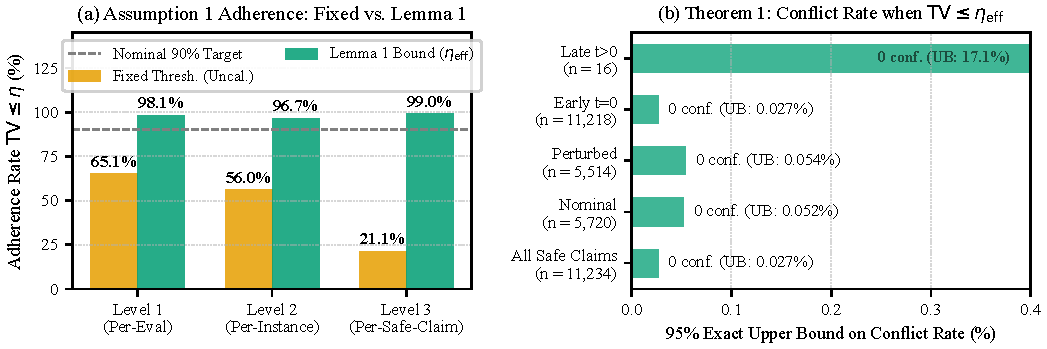
\includegraphics[width=\columnwidth,keepaspectratio]{static/images/fig_theorem1_assumption1}
\caption{Empirical evaluation of Theorem~1 and Assumption~1 Total Variation ($\mathrm{TV}$) adherence across operational regimes ($n = \aeSafeClaimsTotal$ safe-claim commitments, \aeTotalTvObservations\ total $\mathrm{TV}$ observations). (Left) Assumption~1 $\mathrm{TV}$ adherence across evaluation, instance, and claim levels under Lemma~1 drift bound $\eta_{\text{eff}}$ relative to the \aeAdherenceIdealThreshold\% target line, contrasted with the historical pre-calibration baseline snapshot (\aeFixedThresholdAdherence\%). (Right) Empirical safe-claim conflict rate (\aeZeroConflicts/\aeSafeClaimsAdhered\ conflicts when $\mathrm{TV} \le \eta_{\text{eff}}$, one-sided \aeConfidenceLevel\% Clopper--Pearson exact upper bound \aeTheoremConflictRateUpper\%).}
\label{fig:theorem1_assumption1}
\end{figure}

\begin{theorem}[Finite-Time Consensus Stabilization and Oscillation-Freedom]
Consider Phase~2 consensus for task $j$ under subjective beliefs $B_r, B_s \in \Delta(\Theta)$ with initial bid valuations bounded above by $C_{\max} < \infty$:
\begin{enumerate}
    \item \textbf{Limit Cycle in Standard CBBA:} Standard CBBA without margin can enter a cyclic outbidding limit cycle when there exist subjective beliefs satisfying $0 < |c_r(j \mid B_r) - c_s(j \mid B_s)| < L_j \mathrm{TV}(B_r, B_s)$, where $L_j = \max_{q \in \mathcal{R}} L_{q, j}$.
    \item \textbf{Stabilization under Hysteresis Deadband:} Equipping Phase~2 consensus with belief hysteresis deadband $\kappa_{\text{hyst}} m_{r,s,j}$ (where robot $s$ outbids incumbent $r$ only if $\hat{c}_s^s(j) + \kappa_{\text{hyst}} m_{r,s,j} < \hat{c}_r^r(j)$) strictly eliminates outbidding limit cycles. For contested tasks with belief sensitivity $m_{r,s,j} \ge m_{\min} > 0$, outbidding occurs at most $K_{\max} = \lfloor C_{\max} / (\kappa_{\text{hyst}} m_{\min}) \rfloor$ times, bounding quiescent stabilization to $\mathcal{O}(K_{\max} |\mathcal{T}| \cdot \mathrm{diam}(\mathcal{G}_{\text{comm}}))$ communication rounds ($\mathcal{O}(|\mathcal{T}| \cdot \mathrm{diam}(\mathcal{G}_{\text{comm}}))$ when $K_{\max} = \mathcal{O}(1)$). In the degenerate zero-margin case ($m_{r,s,j} = 0$), valuations are belief-invariant and consensus stabilizes in a single wave of $\mathrm{diam}(\mathcal{G}_{\text{comm}})$ rounds.
\end{enumerate}
\label{thm:stabilization}
\end{theorem}
\begin{proof}
Part 1 (Limit Cycle): Suppose $c_r(j \mid B_r) < c_s(j \mid B_r)$, but $c_s(j \mid B_s) < c_r(j \mid B_s)$. If robot $r$ claims task $j$ with bid $c_r(j \mid B_r)$, then over delay $\Delta t$, $s$ evaluates $c_s(j \mid B_s) < c_r(j \mid B_r)$ and outbids $r$ with a newer timestamp. Robot $r$ re-evaluates under $B_r$, finding $c_r(j \mid B_r) < c_s(j \mid B_s)$, and outbids $s$ again, inducing an infinite oscillation of period $2 \Delta t$.

Part 2 (Hysteresis Stabilization): Incumbent winner $r$ has bid $\hat{c}_r^r(j)$; peer $s$ outbids $r$ only if $\hat{c}_s^s(j) + \kappa_{\text{hyst}} m_{r,s,j} < \hat{c}_r^r(j)$.
\textit{Zero-margin case ($m_{r,s,j} = 0$):} Occurs only when $L_{r,j} = L_{s,j} = 0$ and $\delta_{\text{map}} = 0$. By Proposition~\ref{prop:tight_lipschitz}, task valuation is belief-invariant ($\hat{c}_q^q(j) = c_q(j \mid B_r) = c_q(j \mid B_s)$); hence no belief-induced preference reversal occurs, and standard CBBA with deterministic tie-breaking resolves task $j$ in a single consensus wave of $\mathrm{diam}(\mathcal{G}_{\text{comm}})$ communication rounds.
\textit{Positive-margin case ($m_{r,s,j} \ge m_{\min} > 0$):} Within deadband $|\hat{c}_s^s(j) - \hat{c}_r^r(j)| \le \kappa_{\text{hyst}} m_{r,s,j}$, bid disparity is statistically indistinguishable from belief divergence; robots retain the incumbent. Outside the deadband, outbidding strictly reduces the winning bid by at least $\kappa_{\text{hyst}} m_{\min} > 0$. Bounded above by $C_{\max} < \infty$ and below by zero, outbidding for task $j$ can occur at most $K_{\max} = \lfloor C_{\max} / (\kappa_{\text{hyst}} m_{\min}) \rfloor$ times. Across $|\mathcal{T}|$ tasks over network diameter $\mathrm{diam}(\mathcal{G}_{\text{comm}})$, consensus converges in at most $\mathcal{O}(K_{\max} |\mathcal{T}| \cdot \mathrm{diam}(\mathcal{G}_{\text{comm}}))$ rounds, eliminating all limit cycles.
\end{proof}

\begin{proposition}[Exponential Re-Auction Message Reduction]
Let $\bar{\pi} = \max_{e \in E_{\text{risk}}} \pi(e) < 1$ denote the maximum edge blockage probability. Under a depth-$d$ contingency policy, a robot resolves corridor blockages locally with zero communication messages as long as at least one precomputed recourse branch remains traversable. The expected message overhead for handling task blockages satisfies:
\begin{equation}
    \mathbb{E}[\text{Msgs}_{\text{ACA}}] \le \sum_{j \in \mathcal{T}} \bar{\pi}^{d+1} \mathcal{O}(|\mathcal{R}| \cdot \mathrm{diam}(\mathcal{G}_{\text{comm}})),
\end{equation}
achieving an exponential reduction by factor $\mathcal{O}(\bar{\pi}^d)$ relative to standard CBBA re-auction overhead $\sum_{j \in \mathcal{T}} \bar{\pi} \mathcal{O}(|\mathcal{R}| \cdot \mathrm{diam}(\mathcal{G}_{\text{comm}}))$.
\label{prop:message_reduction}
\end{proposition}

\section{Experimental Evaluation}

\subsection{Experimental Setup and Benchmark Environments}
All experiments were conducted across five graph topology families, encompassing two real benchmark maps and three synthetic stress-test graph models:

\begin{figure*}[!t]
\centering
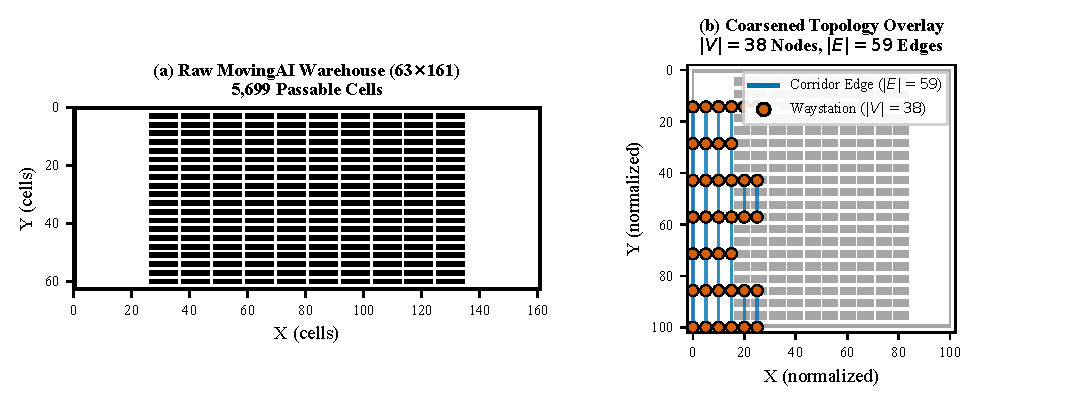
\includegraphics[width=0.62\textwidth,height=2.3cm,keepaspectratio]{static/images/fig_map_movingai_warehouse}%
\hfill
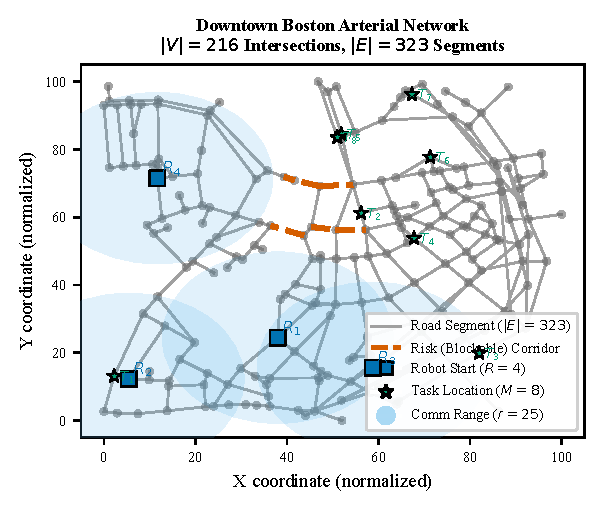
\includegraphics[width=0.35\textwidth,height=2.3cm,keepaspectratio]{static/images/fig_map_boston_road}\\[3pt]
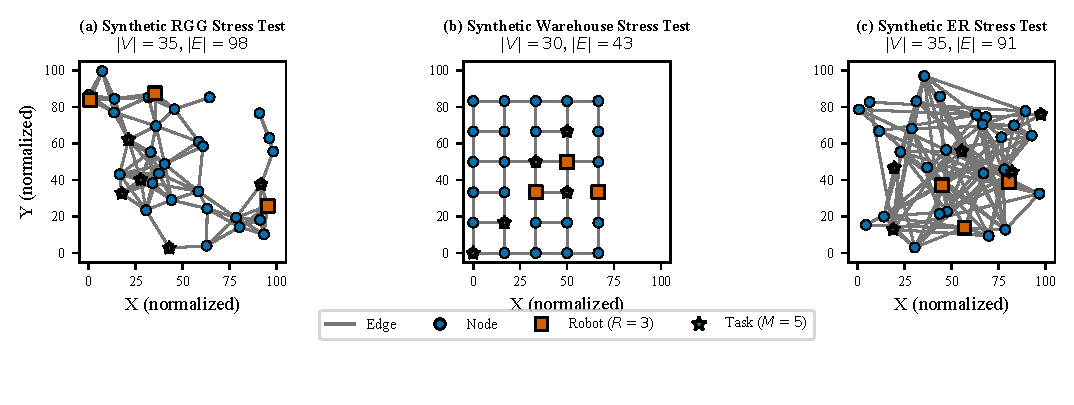
\includegraphics[width=0.98\textwidth,height=2.1cm,keepaspectratio]{static/images/fig_map_synthetic_families}
\caption{Benchmark Navigation Topologies: (Top Left) Real MovingAI warehouse map ($\aeMapMovingAiGridW \times \aeMapMovingAiGridH$ grid, \aeMapMovingAiPassableCells\ passable cells) and coarsened navigation backbone ($n = \aeMapMovingAiNodes, |E| = \aeMapMovingAiBackboneEdges$). (Top Right) Real Downtown Boston road network ($n = \aeMapBostonNodes, |E| = \aeMapBostonEdges$) displaying risk corridors, robot starts ($R = \aeFleetSize$), task locations ($M = \aeBostonTasks$), and communication range ($r_{\mathrm{comm}} = \aeBostonCommRange\text{ m}$, topology-scaled for street density vs.\ nominal $r_{\mathrm{comm}} = \aeCommRange\text{ m}$). (Bottom) Synthetic benchmark families evaluated as stress tests (Random Geometric, Warehouse Grid, Erd\H{o}s--R\'enyi).}
\label{fig:benchmark_maps}
\end{figure*}

\begin{enumerate}[leftmargin=*,itemsep=1pt,topsep=2pt,parsep=0pt]
    \item \textbf{MovingAI Warehouse MAPF Benchmark:} Standard automated storage and retrieval warehouse benchmark (\texttt{warehouse-10-20-10-2-1.map}, \aeMapMovingAiPassableCells\ passable cells, \aeMapMovingAiEdges\ edges) deterministically coarsened by corridor block pooling into $n = \aeMapMovingAiNodes$ waypoint nodes and $|E| = \aeMapMovingAiBackboneEdges$ traversable corridor edges (Fig.~\ref{fig:benchmark_maps}, Top Left).
    \item \textbf{Downtown Boston Road Network:} Real-world street topology extracted via OSMnx (\texttt{boston\_downtown\_drive.graphml}) comprising $n = \aeMapBostonNodes$ street intersections and $|E| = \aeMapBostonEdges$ traversable roadway segments (Fig.~\ref{fig:benchmark_maps}, Top Right).
    \item \textbf{Random Geometric Graphs (RGG):} Metric embedding in $[\aeCoordZero, \aeMapRggSize] \times [\aeCoordZero, \aeMapRggSize]$ ($n = \aeMapRggNodes$, radius $r_c \approx \aeMapRggRadius$).
    \item \textbf{Warehouse Grid Graphs:} Grid layouts with dedicated aisles ($n = \aeMapGridNodes$).
    \item \textbf{Erd\H{o}s-R\'enyi Graphs (ER):} $G(n, p)$ topologies ($n = \aeMapErNodes, p = \aeMapErP$) (Fig.~\ref{fig:benchmark_maps}, Bottom).
\end{enumerate}

We benchmarked ACA against literature baselines, level-execution variants (+LR) with identical detour capability, and clean algorithmic ablations:
\begin{itemize}[leftmargin=*,itemsep=1pt,topsep=2pt,parsep=0pt]
    \item \textbf{CBBA~\cite{choi2009cbba} and CBBA+LR:} Standard Consensus-Based Bundle Algorithm (drops full bundle on blockage) and its level-execution counterpart (+LR) equipped with identical local recourse detour execution.
    \item \textbf{CBBA-PR (Adapted)~\cite{buckman2019partial} and CBBA-PR+LR:} Re-auctions solely the blocked task, preserving the remaining bundle sequence.
    \item \textbf{SSI~\cite{koenig2006ssi} and SSI+LR:} Sequential Single-Item auction with tour-insertion marginal costs and replan on blockage.
    \item \textbf{CTP Replan and Implicit Coordination~\cite{alighanbari2005implicit}:} Canadian Traveller Problem replan-on-discovery policy, and margin-free implicit auction without consensus message rounds.
    \item \textbf{Clairvoyant Greedy (Oracle Reference):} Centralized Hungarian matching on the ground-truth open graph.
    \item \textbf{ACA Ablations:} ACA (No Margin), ACA (Depth \aeDepthZero), ACA (Depth \aeDepthTwo), and ACA (No Inference).
\end{itemize}

\begin{table*}[t]
\centering
\caption{Main Benchmark Results Across Graph Topologies and Adversary Types (Mean $\pm$ 95\% Bootstrap CI, Balanced Core Grid, $N = 750$ Paired Trials per Method Across 250 Independent Instances).
$^\dagger$ denotes statistically significant difference vs.\ ACA ($p < 0.05$, paired Wilcoxon signed-rank test with Holm--Bonferroni correction).}
\label{tab:main_results}
\begin{tabular}{lcccccc}
\toprule
\textbf{Method} & \textbf{Completion (\%)} & \textbf{Net Welfare} & \textbf{Distinct Conf.} & \textbf{Total Conf.} & \textbf{Messages} & \textbf{Tick RT (ms)} \\
\midrule
\textbf{ACA (Ours)} & $90.9 \pm 0.9$ & $921 \pm 22$ & $6.3 \pm 0.2$ & $38.1 \pm 2.3$ & $236 \pm 11$ & $35.52 \pm 2.40$ \\
ACA (No Margin Ablation) & $90.7 \pm 0.9$ & $910 \pm 21$ & $7.8 \pm 0.2$$^\dagger$ & $47.4 \pm 2.6$$^\dagger$ & $238 \pm 10$ & $24.60 \pm 1.59$$^\dagger$ \\
ACA (Depth-0 Ablation) & $86.8 \pm 1.0$$^\dagger$ & $916 \pm 19$ & $6.6 \pm 0.2$$^\dagger$ & $42.0 \pm 2.3$$^\dagger$ & $301 \pm 11$$^\dagger$ & $23.43 \pm 1.22$$^\dagger$ \\
ACA (Depth-2) & $91.2 \pm 0.9$ & $925 \pm 21$ & $6.3 \pm 0.2$ & $38.5 \pm 2.4$ & $234 \pm 10$ & $34.79 \pm 2.27$ \\
ACA (No Inference) & $90.9 \pm 0.9$ & $928 \pm 21$ & $6.3 \pm 0.2$ & $38.7 \pm 2.4$ & $235 \pm 10$ & $31.98 \pm 2.00$$^\dagger$ \\
CBBA \cite{choi2009cbba} & $82.1 \pm 1.2$$^\dagger$ & $879 \pm 19$$^\dagger$ & $8.0 \pm 0.2$$^\dagger$ & $50.4 \pm 2.5$$^\dagger$ & $312 \pm 10$$^\dagger$ & $11.89 \pm 0.63$$^\dagger$ \\
CBBA (+LR) & $88.8 \pm 0.9$$^\dagger$ & $910 \pm 19$ & $7.9 \pm 0.2$$^\dagger$ & $50.6 \pm 2.7$$^\dagger$ & $263 \pm 10$$^\dagger$ & $12.67 \pm 0.70$$^\dagger$ \\
CBBA-PR (Adapted) \cite{buckman2019partial} & $90.4 \pm 0.9$ & $977 \pm 17$$^\dagger$ & $8.0 \pm 0.2$$^\dagger$ & $59.7 \pm 3.2$$^\dagger$ & $295 \pm 12$$^\dagger$ & $12.57 \pm 0.67$$^\dagger$ \\
CBBA-PR (+LR) & $90.3 \pm 0.9$ & $923 \pm 19$ & $7.9 \pm 0.2$$^\dagger$ & $50.1 \pm 2.7$$^\dagger$ & $245 \pm 11$$^\dagger$ & $12.77 \pm 0.70$$^\dagger$ \\
SSI \cite{koenig2006ssi} & $84.3 \pm 1.4$$^\dagger$ & $694 \pm 27$$^\dagger$ & $0.0 \pm 0.0$$^\dagger$ & $0.0 \pm 0.0$$^\dagger$ & $252 \pm 11$ & $12.33 \pm 0.69$$^\dagger$ \\
SSI (+LR) & $84.1 \pm 1.4$$^\dagger$ & $635 \pm 29$$^\dagger$ & $0.0 \pm 0.0$$^\dagger$ & $0.0 \pm 0.0$$^\dagger$ & $214 \pm 10$$^\dagger$ & $12.79 \pm 0.76$$^\dagger$ \\
CTP Replan & $96.4 \pm 0.5$$^\dagger$ & $832 \pm 27$$^\dagger$ & $0.0 \pm 0.0$$^\dagger$ & $0.0 \pm 0.0$$^\dagger$ & $77 \pm 3$$^\dagger$ & $11.64 \pm 0.66$$^\dagger$ \\
Implicit (No Consensus) \cite{alighanbari2005implicit} & $94.5 \pm 0.7$$^\dagger$ & $781 \pm 22$$^\dagger$ & $10.6 \pm 0.2$$^\dagger$ & $107.7 \pm 4.4$$^\dagger$ & $0 \pm 0$$^\dagger$ & $19.57 \pm 1.09$$^\dagger$ \\
Clairvoyant greedy (reference, not a bound) & $96.9 \pm 0.5$$^\dagger$ & $925 \pm 27$$^\dagger$ & $0.0 \pm 0.0$$^\dagger$ & $0.0 \pm 0.0$$^\dagger$ & $0 \pm 0$$^\dagger$ & $15.89 \pm 0.86$$^\dagger$ \\
\bottomrule
\end{tabular}
\end{table*}

\subsection{Quantitative Results and Statistical Analysis}
Table~\ref{tab:main_results} reports quantitative performance across $N = \aeMatchedBenchmarkInstances$ matched benchmark trials (\aeSeedsCount\ seeds $\times$ \aeBenchmarkMapCount\ graph families = \aeBenchmarkClusters\ independent map-seed instances $\times$ \aeAdversaryCount\ in-model adversary types; \aeCoreTrials\ total balanced core trials across fourteen methods). Net Welfare is defined as $\text{Net Welfare} = \sum_{j \in \mathcal{T}_{\text{comp}}} R_j - \sum_{r \in \mathcal{R}} \text{dist}_r$, directly penalizing redundant transit distance. Every cell reports the sample mean and two-sided \aeConfidenceLevel\% cluster bootstrap confidence interval (\aeBootstrapResamples\ resamples). Statistically significant differences vs.~ACA ($p < \aeAlphaSignificance$, cluster-level paired $t$-test with Holm--Bonferroni correction across \aeBenchmarkClusters\ independent map--seed clusters) are designated with $\dagger$. The omnibus Critical Difference diagram (Fig.~\ref{fig:critical_difference_diagram}) establishes algorithm ranking clusters across benchmark topologies under Nemenyi post-hoc analysis.

\begin{figure}[!htbp]
\centering
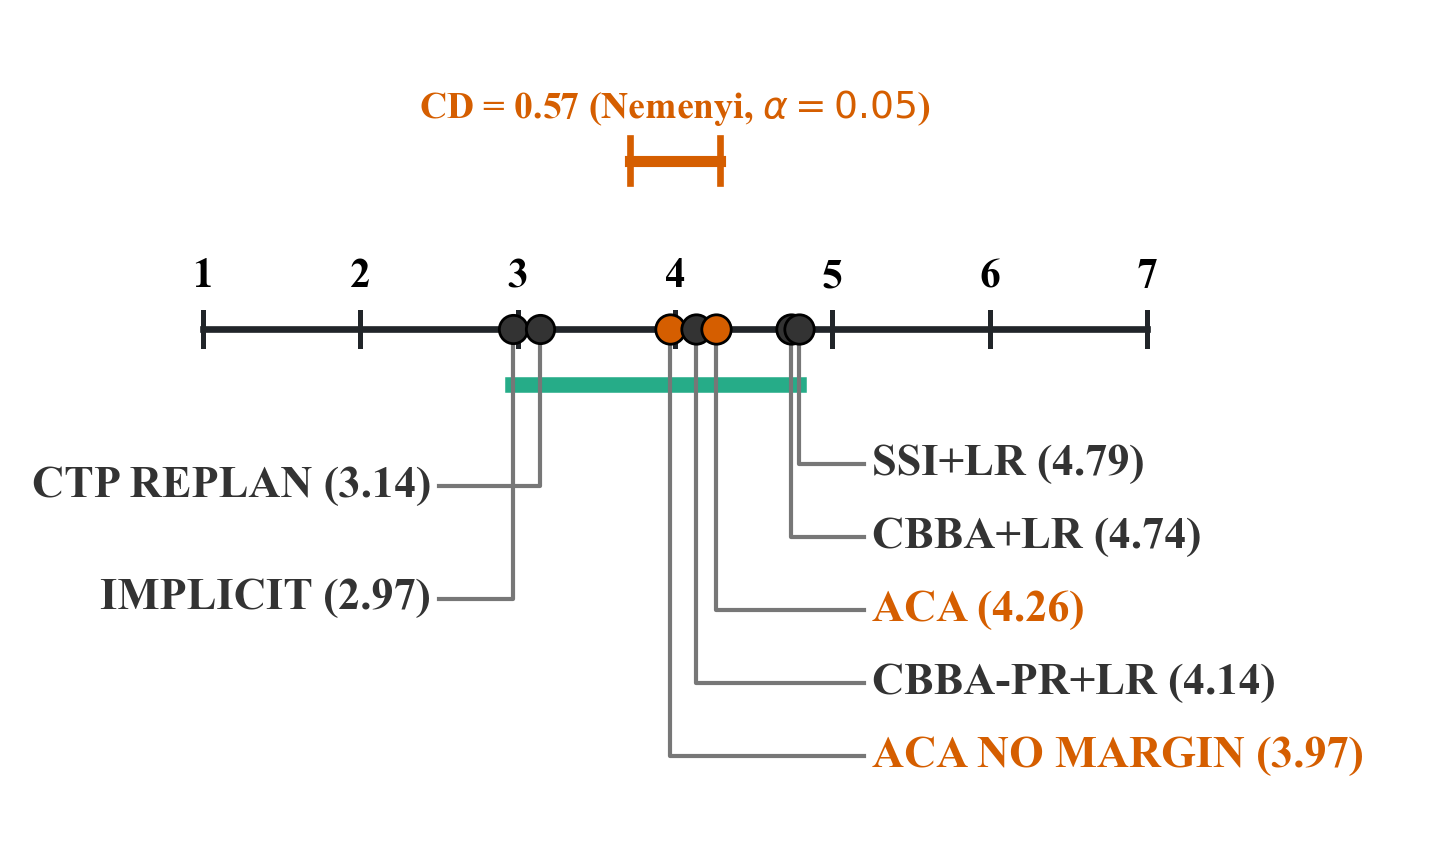
\includegraphics[width=0.68\columnwidth,keepaspectratio]{static/images/fig_critical_difference_diagram.png}
\caption{Critical Difference (CD) diagram for algorithm completion rankings across benchmark topologies ($N = \aeMatchedBenchmarkInstances$ matched benchmark trials across \aeBenchmarkClusters\ independent map-seed instances). Statistical differences evaluated via omnibus Friedman rank-sum test ($\chi^2_F = \aeFriedmanChiSq, p < 10^{-15}$) with post-hoc Nemenyi critical difference analysis at $\alpha = \aeAlphaSignificance$; horizontal bars connect algorithms with statistically indistinguishable performance rankings.}
\label{fig:critical_difference_diagram}
\end{figure}

\subsubsection{Gains over Standard CBBA}
Under persistent corridor blockages, standard CBBA drops its entire bundle upon a single blockage and initiates fleet-wide market re-auctions. Consequently, standard CBBA achieves only $\aeCbbaComp \pm \aeCbbaCompCI\%$ completion while exchanging $\aeCbbaMsgs \pm \aeCbbaMsgsCI$ messages. By contrast, ACA leverages type-aware expected recourse cost valuation and zero-message local detour execution, achieving $\aeAcaComp \pm \aeAcaCompCI\%$ completion ($\aeCompletionDiffCbba$ percentage points, $p < \aeAlphaSignificance$, Cliff's $\delta = \aeCliffsDeltaCbba$) and exchanging $\aeAcaMsgs \pm \aeAcaMsgsCI$ messages (a significant reduction of $\aeMsgDiffCbba$ messages, $p < \aeAlphaSignificance$).

\subsubsection{Headline Comparison: ACA vs. CBBA+LR}
To isolate the benefit of ACA's market mechanism beyond raw detour execution, our primary headline comparison evaluates ACA against CBBA equipped with identical local recourse (+LR). ACA achieves a statistically significant completion gain of \aeHtwoCbbaLrDiff\ percentage points over CBBA+LR (Hodges--Lehmann median difference \aeHtwoCbbaLrHlMedian~pp, \aeConfidenceLevel\% CI [\aeHtwoCbbaLrCILow, \aeHtwoCbbaLrCIHigh]~pp, $p < \aePvalCbbaLr$). This establishes that contingency-aware bidding and safe-claim margin calculation provide measurable coordination benefits beyond simple reactive detour execution.

\begin{table}[htbp]
\centering
\caption{Software-in-the-Loop (SITL) Physics Simulation vs.\ Discrete Graph Simulation ($N = 360$ total trials across 60 paired physical instances per method on real maps). $p$-val evaluates paired completion difference vs.\ ACA (paired Wilcoxon signed-rank test with Holm--Bonferroni multiple-testing correction across baselines).}
\label{tab:sitl_results}
\renewcommand{\arraystretch}{0.92}
\resizebox{\columnwidth}{!}{%
\begin{tabular}{@{\hskip 2pt}l@{\hskip 3pt}c@{\hskip 3pt}c@{\hskip 3pt}c@{\hskip 3pt}c@{\hskip 3pt}c@{\hskip 3pt}c@{\hskip 3pt}c@{}}
\toprule
\textbf{Method} & \textbf{SITL (\%)} & \textbf{Graph (\%)} & \textbf{Gap (pp)} & \textbf{Net Welfare} & \textbf{Contacts} & \textbf{Conflicts} & \textbf{$p$-val} \\
\midrule
\textbf{ACA (Ours)} & 69.4 $\pm$ 20.3 & 88.4 $\pm$ 16.7 & -18.9 & 261 $\pm$ 18 & 158.6 $\pm$ 36.2 & 37.5 $\pm$ 3.5 & -- \\
ACA (No Margin Ablation) & 68.6 $\pm$ 20.4 & 88.6 $\pm$ 14.9 & -20.1 & 224 $\pm$ 18 & 171.7 $\pm$ 40.2 & 66.5 $\pm$ 5.0 & 0.8358 \\
CBBA-PR (+LR) & 68.8 $\pm$ 19.4 & 90.3 $\pm$ 13.7 & -21.5 & 222 $\pm$ 18 & 194.7 $\pm$ 41.2 & 70.0 $\pm$ 5.3 & 0.8358 \\
CTP Replan & 68.4 $\pm$ 20.8 & 91.3 $\pm$ 15.7 & -22.9 & 263 $\pm$ 20 & 142.3 $\pm$ 38.0 & 0.0 & 0.8358 \\
Implicit (No Consensus) \cite{alighanbari2005implicit} & 74.9 $\pm$ 19.5 & 92.1 $\pm$ 13.7 & -17.2 & 159 $\pm$ 21 & 199.8 $\pm$ 41.9 & 168.6 $\pm$ 3.8 & $< 10^{-4}$ \\
SSI (+LR) & 42.2 $\pm$ 25.4 & 72.2 $\pm$ 30.1 & -30.1 & 133 $\pm$ 18 & 143.6 $\pm$ 34.4 & 0.0 & $< 10^{-4}$ \\
\bottomrule
\end{tabular}%
}
\end{table}

\subsubsection{Ablation Analysis: Recourse, Margin, and Inference}
To isolate the distinct mechanisms in ACA, we analyzed three clean ablations shown in Fig.~\ref{fig:ablation_suite}:
\begin{itemize}[leftmargin=*,itemsep=0pt,topsep=1pt,parsep=0pt]
    \item \textbf{Recourse Depth Ablation (ACA Depth-\aeRecourseDepthZero):} Disabling contingency recourse ($d = \aeRecourseDepthZero$) while retaining the Pinsker margin drops completion from $\aeAcaComp \pm \aeAcaCompCI\%$ down to $\aeAcaDepthZeroComp \pm \aeAcaDepthZeroCompCI\%$ (mean diff \aeHoneMeanDiff~pp, HL median \aeHoneHlMedian~pp, adjusted $p < 10^{-10}$) and increases messages to $\aeAcaDepthZeroMsgs \pm \aeAcaDepthZeroMsgsCI$, confirming recourse is essential under persistent blockages.
    \item \textbf{Margin Ablation (ACA No Margin):} Evaluating ACA without the Pinsker margin yields $\aeAcaNoMarginComp \pm \aeAcaNoMarginCompCI\%$ completion and $\aeAcaNoMarginTotConf \pm \aeAcaNoMarginTotConfCI$ total conflicts. In Phase~1, safe claims eliminate conflicts by \aeHfourSafeConflictReductionPct\% vs.\ No Margin (reducing conflicts from \aeNoMarginSafeConflicts\ down to \aeTotalSafeConflicts, achieving \aeConflictFreeRunPct\% conflict-free runs; $\aeTotalSafeConflictsMean \pm \aeTotalSafeConflictsCI$ vs.\ $\aeNoMarginSafeConflictsMean \pm \aeNoMarginSafeConflictsCI$, $p < 10^{-40}$) with non-inferior welfare ($p = \aePvalHthreeWelfare$). Under Theorem~1, when $D_{\mathrm{TV}} \le \eta_{\mathrm{eff}}$, Phase-1 safe-claim conflicts are zero (\aeTheoremConflicts\ conflicts across \aeSafeClaimsAdhered\ adhered claims; \aeConfidenceLevel\% Clopper--Pearson exact upper bound \aeTheoremConflictRateUpper\%), while distinct task conflicts drop from $\aeAcaNoMarginDistConf \pm \aeAcaNoMarginDistConfCI$ down to $\aeAcaDistConf \pm \aeAcaDistConfCI$ ($p < \aeAlphaSignificance$) and total consensus conflicts maintain statistical parity ($\aeAcaTotConf \pm \aeAcaTotConfCI$ vs.\ $\aeAcaNoMarginTotConf \pm \aeAcaNoMarginTotConfCI$).
    \item \textbf{Bayesian Type Inference Parity and Specialization (ACA No Inference):} Robots evaluate depth-\aeRecourseDepthOne\ contingency trees under online Bayesian updates or a static uniform prior (ACA No Inference). Under homogeneous hazards, depth-\aeRecourseDepthOne\ recourse trees hedge against failures even under a uniform prior ($\aeAcaComp \pm \aeAcaCompCI\%$ vs.\ $\aeNoInfComp \pm \aeNoInfCompCI\%$, HL diff \aeHfiveHlMedian~pp, $p = \aePvalInferenceNull$, Fig.~\ref{fig:ablation_suite}b). In contrast, under structurally partitioned vulnerabilities ($E_{\text{risk}}^{\theta}$, $N = \aePartitionedInstances$ matched instances across \aeBenchmarkMapCount\ topologies), Bayesian inference concentrates posterior mass $B_r(\theta^*) \to 1$ on the active threat, achieving $\aePartitionedAcaComp \pm \aePartitionedAcaCompCI\%$ completion ($\aePartitionedAcaWelfare \pm \aePartitionedAcaWelfareCI$ welfare) and outperforming CBBA+LR across all threat regimes: \aePartitionedThetaOneDiff~pp on $\theta_1$ (\aePartitionedThetaOneAca\% vs.\ \aePartitionedThetaOneCbbaLr\%), \aePartitionedThetaTwoDiff~pp on $\theta_2$ (\aePartitionedThetaTwoAca\% vs.\ \aePartitionedThetaTwoCbbaLr\%), and \aePartitionedThetaThreeDiff~pp on $\theta_3$ (\aePartitionedThetaThreeAca\% vs.\ \aePartitionedThetaThreeCbbaLr\%, $p < 10^{-20}$). Theorem~1 holds across this sweep: ACA maintains $\aePartitionedAcaSafeConf \pm \aePartitionedAcaSafeConfCI$ Phase-1 safe-claim conflicts (vs.\ $\aePartitionedNoMarginSafeConf \pm \aePartitionedNoMarginSafeConfCI$ for No Margin, $p < 10^{-50}$), preserves Phase-2 consensus conflict parity ($\aePartitionedAcaConsConf \pm \aePartitionedAcaConsConfCI$ vs.\ $\aePartitionedNoMarginConsConf \pm \aePartitionedNoMarginConsConfCI$; \aePartitionedThetaThreeAcaConsConf\ vs.\ \aePartitionedThetaThreeNoMarginConsConf\ on $\theta_3$), and reduces communication by \aePartitionedMsgReductionPct\% ($p < 10^{-5}$). Because uniform marginals $\pi_{\text{unif}}(e) = \aePartitionedUniformMarginal$ fall below threshold $\tau_{\text{prune}} = \aePartitionedPruneThreshold$, unspecialized agents cannot execute zero-message detours, inducing partial re-auctions upon blockages.
\end{itemize}

\begin{figure}[!htbp]
\centering
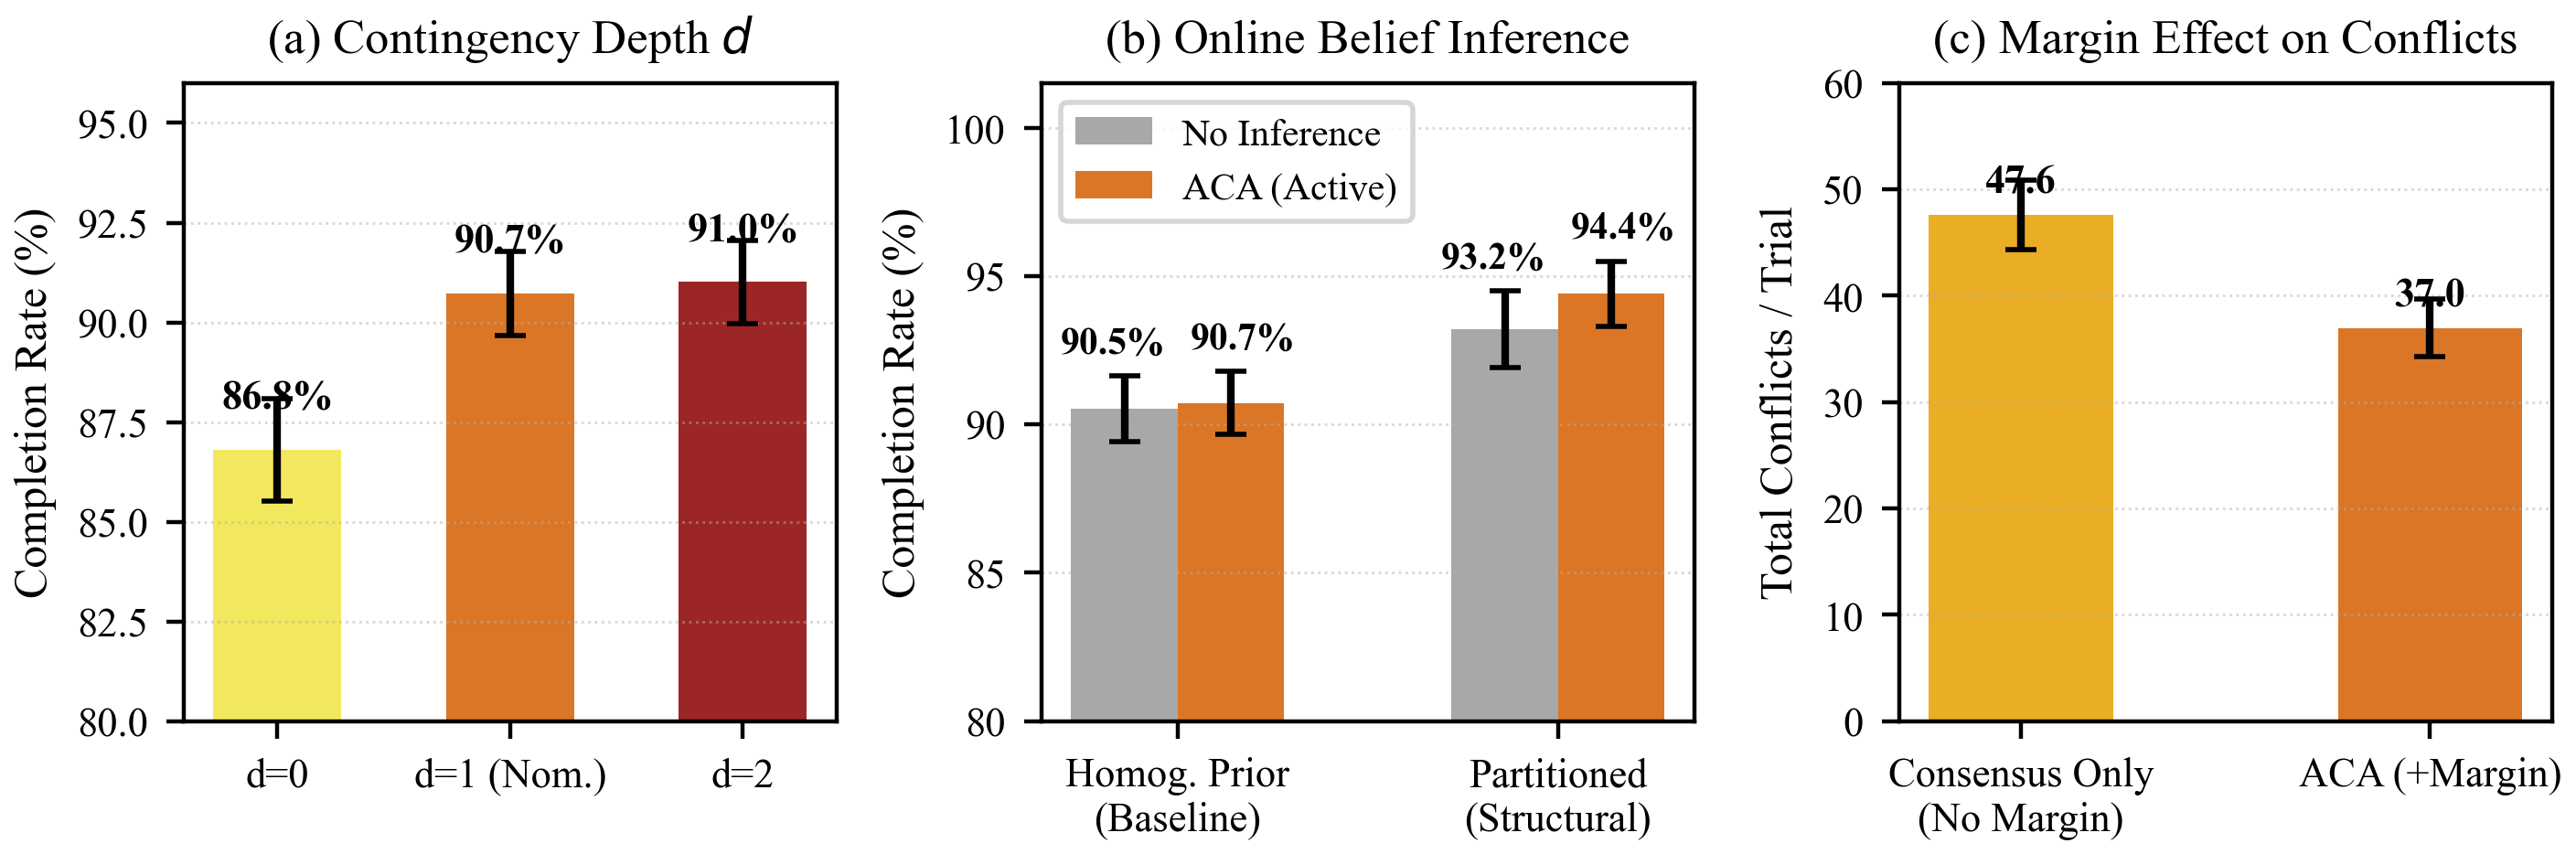
\includegraphics[width=0.85\columnwidth,keepaspectratio]{static/images/fig_ablation_suite.png}
\caption{Systematic ablation analysis of ACA core algorithmic mechanisms ($N = \aeMatchedBenchmarkInstances$ matched benchmark trials across \aeBenchmarkClusters\ independent map-seed instances per baseline ablation condition, plus $N = \aePartitionedInstances$ structurally partitioned evaluation instances). Panels depict: (Left) Recourse depth ablation ($d=\aeRecourseDepthZero$ vs. $d=\aeRecourseDepthOne$, paired Wilcoxon test $p < 10^{-10}$); (Center) Online Bayesian type inference vs.\ static uniform prior under homogeneous hazards ($p = \aePvalInferenceNull$) and partitioned vulnerabilities ($p < 10^{-5}$); (Right) Pinsker margin ablation and conflict reduction ($p < \aeAlphaSignificance$).}
\label{fig:ablation_suite}
\end{figure}

\subsubsection{Baseline Trade-offs and Parameter Sensitivity}
\begin{itemize}[leftmargin=*,itemsep=0pt,topsep=1pt,parsep=0pt]
    \item \textbf{CBBA-PR~\cite{buckman2019partial}:} Re-auctions solely the blocked task ($\aeCbbaPartialWelfare \pm \aeCbbaPartialWelfareCI$ welfare), but incurs \aeCbbaPartialConfIncreasePct\% more conflicts ($\aeCbbaPartialTotConf \pm \aeCbbaPartialTotConfCI$) and \aeCbbaPartialMsgIncreasePct\% more messages ($\aeCbbaPartialMsgs \pm \aeCbbaPartialMsgsCI$). With recourse (CBBA-PR+LR), ACA matches completion while reducing conflicts.
    \item \textbf{CTP Replan and Implicit Coordination~\cite{alighanbari2005implicit}:} Greedy heuristics clear tasks before cutoff by dispatching multiple robots redundantly ($\aeImplicitTotConf \pm \aeImplicitTotConfCI$ conflicts for Implicit), severely penalizing Net Welfare ($\aeCtpWelfare \pm \aeCtpWelfareCI$ and $\aeImplicitWelfare \pm \aeImplicitWelfareCI$ vs.\ ACA's $\aeAcaWelfare \pm \aeAcaWelfareCI$, $p < \aeAlphaSignificance$).
    \item \textbf{Sequential Single-Item (SSI):} SSI achieves completion $\aeSsiComp \pm \aeSsiCompCI\%$ with zero conflicts but low net welfare ($\aeSsiWelfare \pm \aeSsiWelfareCI$). With recourse (SSI+LR), ACA maintains an advantage of \aeHtwoSsiLrDiff~pp ($p < 10^{-5}$).
    \item \textbf{Clairvoyant Greedy (Oracle Reference):} Centralized omniscient Oracle achieves $\aeOracleComp \pm \aeOracleCompCI\%$ completion and $\aeOracleWelfare \pm \aeOracleWelfareCI$ welfare with zero conflicts, serving as an empirical reference.
    \item \textbf{Out-of-Model Adversary ($\theta_4$) and Sweeps:} Across the \aeTotalTrials-trial sweep spanning out-of-model cyclic patrol ($\theta_4 \notin \Theta$), budgets $k \in \{\aeKappaTwo, \aeKappaFour, \aeKappaSix\}$, and lossy channels, ACA maintains completion and conflict advantages without filter divergence.
\end{itemize}
Mean per-tick computation time for ACA is $\aeAcaRuntime \pm \aeAcaRuntimeCI$ ms, operating within real-time multi-robot planning rates while executing contingency tree evaluation and Theory of Mind calculations.

\subsection{Software-in-the-Loop Simulation in PyBullet}
To evaluate algorithmic conclusions under continuous physical execution, we conducted Software-in-the-Loop (SITL) simulations using PyBullet rigid-body physics, Reciprocal Velocity Obstacles (RVO) avoidance, and OpenCV ArUco tracking across $N = \aeSitlMatchedTrials$ trials across \aeSitlPhysicalInstances\ paired physical instances per method (\aeSitlMethodsCount\ methods, Table~\ref{tab:sitl_results}).

\noindent\textbf{1) Continuous Physics and Domain Gap:} Turning radii and congestion induce a completion gap of \aeSitlDomainGap~pp for ACA (\aeSitlGraphComp\% discrete vs.\ \aeSitlAcaComp\% continuous). Despite this, ACA achieves highest net welfare among decentralized auctions ($\aeSitlAcaWelfare \pm \aeSitlAcaWelfareCI$), outperforming ACA No Margin ($\aeSitlNoMarginWelfare \pm \aeSitlNoMarginWelfareCI$), CBBA-PR+LR ($\aeSitlCbbaPrLrWelfare \pm \aeSitlCbbaPrLrWelfareCI$), SSI+LR ($\aeSitlSsiLrWelfare \pm \aeSitlSsiLrWelfareCI$), and Implicit Coordination ($\aeSitlImplicitWelfare \pm \aeSitlImplicitWelfareCI$, all $p < \aeAlphaSignificance$; CTP Replan: $\aeSitlCtpWelfare \pm \aeSitlCtpWelfareCI$).

\noindent\textbf{2) Collision Avoidance, Contacts, and Perception:} Continuous RVO avoidance and corridor traffic induce physical contacts ($\aeSitlAcaContacts \pm \aeSitlAcaContactsCI$ for ACA vs.\ $\aeSitlNoMarginContacts \pm \aeSitlNoMarginContactsCI$ for No Margin, $\aeSitlCbbaPrLrContacts \pm \aeSitlCbbaPrLrContactsCI$ for CBBA-PR+LR, and $\aeSitlImplicitContacts \pm \aeSitlImplicitContactsCI$ for Implicit). Crucially, ACA's recourse and Pinsker margin achieve significantly fewer discrete conflicts ($\aeSitlAcaConflicts \pm \aeSitlAcaConflictsCI$) than No Margin ($\aeSitlNoMarginConflicts \pm \aeSitlNoMarginConflictsCI$), CBBA-PR+LR ($\aeSitlCbbaPrLrConflicts \pm \aeSitlCbbaPrLrConflictsCI$), and Implicit ($\aeSitlImplicitConflicts \pm \aeSitlImplicitConflictsCI$, $p < \aeAlphaSignificance$). Closed-loop ArUco vision perception on barricades achieved \aeVisionDetectionRate\% detection rate ($[\aeVisionDetectionRateCILow\%, \aeVisionDetectionRateCIHigh\%]$) with mean position error $\aeVisionPositionError$~m ($[\aeVisionPositionErrorCILow, \aeVisionPositionErrorCIHigh]$~m) and orientation error $\aeVisionOrientationError$~rad ($\aeVisionOrientationDeg^\circ$), validating robustness to perceptual noise and motion blur.

\section{Limitations and Future Work}
(1)~\textit{Hardware Testbeds:} Physical multi-robot deployments remain future work. (2)~\textit{Extended Partitions:} When $\Delta t_{r,s} \gg 1$, drift $\eta_{\text{eff}} \to 1$ inflates margin $m_{r,j}$, deferring Phase-1 claims to consensus. (3)~\textit{Tree Scalability:} Recourse trees scale with depth $d$; practical deployments employ pruning ($d \in \{\aeDepthOne, \aeDepthTwo\}$).

\section{Conclusion}
We presented Adversarial Contingency Auctions (ACA) for decentralized multi-robot task allocation under strategic blockages and belief divergence. By combining type-aware expected recourse valuation with an analytical Pinsker margin and consensus hysteresis deadband, ACA provably guarantees zero simultaneous Phase-1 conflicts under bounded belief drift and eliminates outbidding cycles. Across $N = \aeMatchedBenchmarkInstances$ matched benchmark trials (\aeBenchmarkClusters\ independent instances) and closed-loop PyBullet physics ($N = \aeSitlMatchedTrials$ trials), ACA demonstrated significant completion gains over CBBA (\aeCompletionDiffCbba~pp) and CBBA+LR (\aeHtwoCbbaLrDiff~pp, $p < \aePvalCbbaLr$), reduced safe conflicts by \aeHfourSafeConflictReductionPct\% (\aeConflictFreeRunPct\% conflict-free runs), and achieved highest net welfare in physical simulation ($\aeSitlAcaWelfare \pm \aeSitlAcaWelfareCI$, $p < \aeAlphaSignificance$) with \aeSitlConflictReductionNoMarginPct\%--\aeSitlConflictReductionCbbaPrLrPct\% fewer conflicts.

\def\BIBdecl{\setlength{\itemsep}{0pt plus 0.2pt}\setlength{\parsep}{0pt}}
\bibliographystyle{IEEEtran}
\bibliography{references}

\end{document}
